\documentclass[14pt,a4paper]{extarticle}

\usepackage[T1]{fontenc}
\usepackage[utf8]{inputenc}
\usepackage[polish]{babel}
\usepackage{lmodern}
\usepackage[hidelinks]{hyperref}
\usepackage{geometry}
\usepackage{graphicx}
\usepackage{amsmath}
\usepackage{pgfplots}
\usepackage{float}
\usepackage[table]{xcolor}
\usepackage{array}
\usepackage{fancyhdr}
\pgfplotsset{compat=1.18}
\geometry{margin=2.5cm}
\setlength{\headheight}{17pt}

\begin{document}

% Front page
\begin{titlepage}
    \thispagestyle{empty}
    \centering

    \vspace*{1.1cm}
    \includegraphics[width=0.82\textwidth]{/Users/marcinpawlak/.cursor/projects/Users-marcinpawlak-Documents-STUDIA-SEM-2-minimaps/assets/logo_MINI_big-5f89496c-f82a-435b-8820-91ad95cd2a18.png}\par

    \vspace{1.7cm}
    {\fontsize{20}{24}\selectfont\textsc{Podstawy Teorii Informacji}\par}

    \vspace{1.0cm}
    {\Large Laboratorium 1\par}

    \vspace{0.25cm}
    {\large Raport projektowy MiniMaps\par}

    \vspace{1.1cm}
    \rule{0.9\textwidth}{0.5pt}
    \vspace{0.55cm}

    {\LARGE\bfseries
    MiniMaps - Raport 1
    \par}

    \vspace{0.55cm}
    \rule{0.9\textwidth}{0.5pt}

    \vfill
    {\Large \textbf{Autorzy}\par}
    \vspace{0.25cm}
    {\large
    Goran Pangełow\par
    Marcin Pawlak\par
    Mikołaj Pesta\par
    Ignacy Drężek\par
    Iga Oleksiewicz\par
    Maks Młynarczyk\par}

    \vspace{0.45cm}
    {\large 21 marca 2026\par}
\end{titlepage}

% Contents page
\tableofcontents
\clearpage

% Header and footer style (excluding title page)
\pagestyle{fancy}
\fancyhf{}
\lhead{\footnotesize Podstawy Teorii Informacji}
\rhead{\footnotesize ETAP I}
\lfoot{\footnotesize Wydział Matematyki i Nauk Informacyjnych}
\rfoot{\footnotesize \thepage}
\renewcommand{\headrulewidth}{0.4pt}
\renewcommand{\footrulewidth}{0.4pt}

\section{Wstęp, motywacja i opis raportu}

Celem naszego projektu jest stworzenie kompleksowej mapy kampusu Politechniki Warszawskiej na wzór popularnych Google Maps. Naszą motywacją są osobiste przeżycia z pierwszych tygodni jako studentów PW, jak i późniejszych prób odnalezienia się na nieznanych nam wydziałach, np. podczas zajęć z Języków Obcych. Nasz pierwszy raport skupia się na rozwijaniu aplikacji w obrębie terenu Wydziału Matematyki i Nauk Informacyjnych i analizie danych, które udało nam się zebrać w trakcie jego realizacji. Raport ten może wydawać się dość chaotyczny, jednak wszystkie zebrane w trakcie jego trwania dane są podstawą do późniejszej implementacji wszystkich założonych przez nas funkcjonalności.

\section{Analiza potrzeb użytkowników i identyfikacja problemów}

\subsection{Metodologia badania pilotażowego}

Aby projektowana aplikacja odpowiadała na rzeczywiste problemy studentów Wydziału MiNI, logikę nawigacyjną oparto na planach ewakuacyjnych budynku, które zostały uzupełnione i zweryfikowane danymi z badania pilotażowego przeprowadzonego na grupie docelowej ($N = 100$ studentów pierwszego roku). Głównym celem zwiadu badawczego była identyfikacja tzw. krytycznych węzłów nawigacyjnych, czyli miejsc, w których architektura gmachu najczęściej wprowadza użytkowników w błąd oraz miejsc, które studenci najczęściej odwiedzają w trakcie ich dnia na uczelni, poza salami dydaktycznymi.

\subsection{Wyniki: Krytyczne węzły nawigacyjne (\textit{ang. pain points - punkty problemowe})}

Zgromadzone dane ilościowe zostały poddane agregacji i przedstawione na poniższym wykresie.

\begin{figure}[htpb]
    \centering
    \begin{tikzpicture}
        \begin{axis}[
            xbar,
            y dir=reverse,
            xlabel={Odsetek studentów wskazujących salę (\%)},
            ylabel={Numer sali dydaktycznej},
            symbolic y coords={313, 107, 303, 216, 215, Inne},
            ytick=data,
            yticklabel style={text width=4.2cm, align=right},
            nodes near coords,
            nodes near coords align={horizontal},
            bar width=18pt,
            width=12cm,
            height=7cm,
            xmin=0, xmax=45,
            title={Wyniki ankiety: Gdzie studenci gubią się najczęściej?},
            grid=major,
            major grid style={dotted, gray}
        ]
        \addplot[fill=red!70!black, draw=black] coordinates {
            (35,313)
            (22,107)
            (18,303)
            (10,216)
            (8,215)
            (7,Inne)
        };
        \end{axis}
    \end{tikzpicture}
    \caption{Rozkład odpowiedzi na pytanie o najtrudniejszą do zlokalizowania salę ($N=100$).}
    \label{fig:trudne_sale}
\end{figure}

\begin{figure}[htpb]
    \centering
    \begin{tikzpicture}
        \begin{axis}[
            xbar,
            y dir=reverse,
            xlabel={Odsetek studentów (\%)},
            ylabel={Miejsce},
            symbolic y coords={Strefa Jet Brains, Bilard, WRS MiNI, Stołówka, Pokój cichej nauki, Inne},
            ytick=data,
            yticklabel style={text width=4.2cm, align=right},
            nodes near coords,
            nodes near coords align={horizontal},
            bar width=14pt,
            width=12cm,
            height=8cm,
            xmin=0, xmax=45,
            title={Wyniki ankiety: Najczęściej na wydziale odwiedzasz?},
            grid=major,
            major grid style={dotted, gray}
        ]
        \addplot[fill=blue!65!black, draw=black] coordinates {
            (38,Strefa Jet Brains)
            (22,Bilard)
            (17,WRS MiNI)
            (10,Stołówka)
            (8,Pokój cichej nauki)
            (5,Inne)
        };
        \end{axis}
    \end{tikzpicture}
    \caption{Wyniki ankiety: Najczęściej odwiedzane miejsca na MiNI poza salami zajęciowymi ($N=100$).}
    \label{fig:miejsca-poza-salami}
\end{figure}

Wykres z ankiety (Rysunek \ref{fig:trudne_sale}) jasno pokazuje jedną rzecz: problemem na MiNI nie jest wcale wielkość gmachu, tylko jego nieintuicyjne zakamarki. Skoro na pierwszym miejscu ląduje sala 313, a zaraz za nią 107 z zupełnie innego piętra, to widać, że studenci nie gubią się ogólnie, tylko w bardzo konkretnych, dziwnych miejscach. Numery pokoi po prostu nie zawsze układają się tak, jak podpowiadałaby logika korytarzy.

Druga ankieta (Rysunek \ref{fig:miejsca-poza-salami}) pokazuje, że życie studenckie na MiNI koncentruje się nie tylko wokół sal dydaktycznych, ale również wokół konkretnych stref wsparcia i odpoczynku. Dominacja strefy Jet Brains oraz wysoki udział billardu wskazują, że studenci regularnie korzystają z przestrzeni sprzyjających zarówno pracy projektowej, jak i krótkiej regeneracji między zajęciami. W kontekście MiNI Maps oznacza to konieczność traktowania tych miejsc jako pełnoprawnych punktów celu w nawigacji: aplikacja powinna umożliwiać ich szybkie wyszukiwanie, przewidywać najczęstsze trasy przejść oraz prezentować je w sposób równie czytelny jak sale zajęciowe.

\subsection{Wnioski dla logiki i architektury systemu}

Wniosek dla naszego projektu jest prosty -- zwykła, płaska mapa z zaznaczoną trasą to za mało. Skoro sam układ korytarzy potrafi zmylić, nasza aplikacja musi być o krok przed użytkownikiem. Jeśli student wyznacza trasę do tej nieszczęsnej sali 313, algorytm nie powinien tylko rysować suchej wektorowej kreski na ekranie.

System musi natychmiast wyłapać, że węzeł docelowy posiada wysoką ,,wagę trudności'' i dorzucić dodatkową podpowiedź. Może to być zdjęcie kłopotliwego rozwidlenia wyświetlane w interfejsie wariantu trasy, albo szybki komunikat tekstowy w stylu: ,,za automatami z kawą skręć w lewo''. Jednocześnie wyniki drugiej ankiety pokazują, że użytkownicy regularnie poruszają się także do miejsc pozadydaktycznych, takich jak strefa Jet Brains czy bilard, więc te punkty również muszą być traktowane jako cele pierwszej kategorii. Krótko mówiąc: nasza nawigacja ma nie tylko łatać błędy w UX (\textit{ang. User Experience - doświadczenie użytkownika}) samego budynku, ale też wspierać codzienne przemieszczanie się między salami i najczęściej odwiedzanymi strefami życia studenckiego.

\section{Podstawy projektowania aplikacji}

\subsection{Plany ewakuacyjne budynku MiNI}
Podstawą projektowania naszych map będą ogólnodostępne w Internecie plany ewakuacyjne Kampusu PW. Takie mapy dobrze oddają ogólny plan budynków, jak i kluczowe dla poprawnego działania aplikacji dokładne rozmieszczenie sal na wydziale. W celu użycia ich w algorytmach optymalizacji tras musimy jednak zastosować metody wektoryzacji, mapując obraz na graf, po którym będziemy mogli swobodnie wykorzystać znane z wielu podobnych projektów metody, jak np. algorytm Dijkstry.

\subsection{Mapa przed i po wektoryzacji}
Poniżej przedstawiono plany ewakuacyjne przed i po procesie wektoryzacji dla każdego piętra Wydziału MiNI.

\begin{figure}[htbp]
    \centering
    \begin{minipage}[t]{0.49\textwidth}
        \centering
        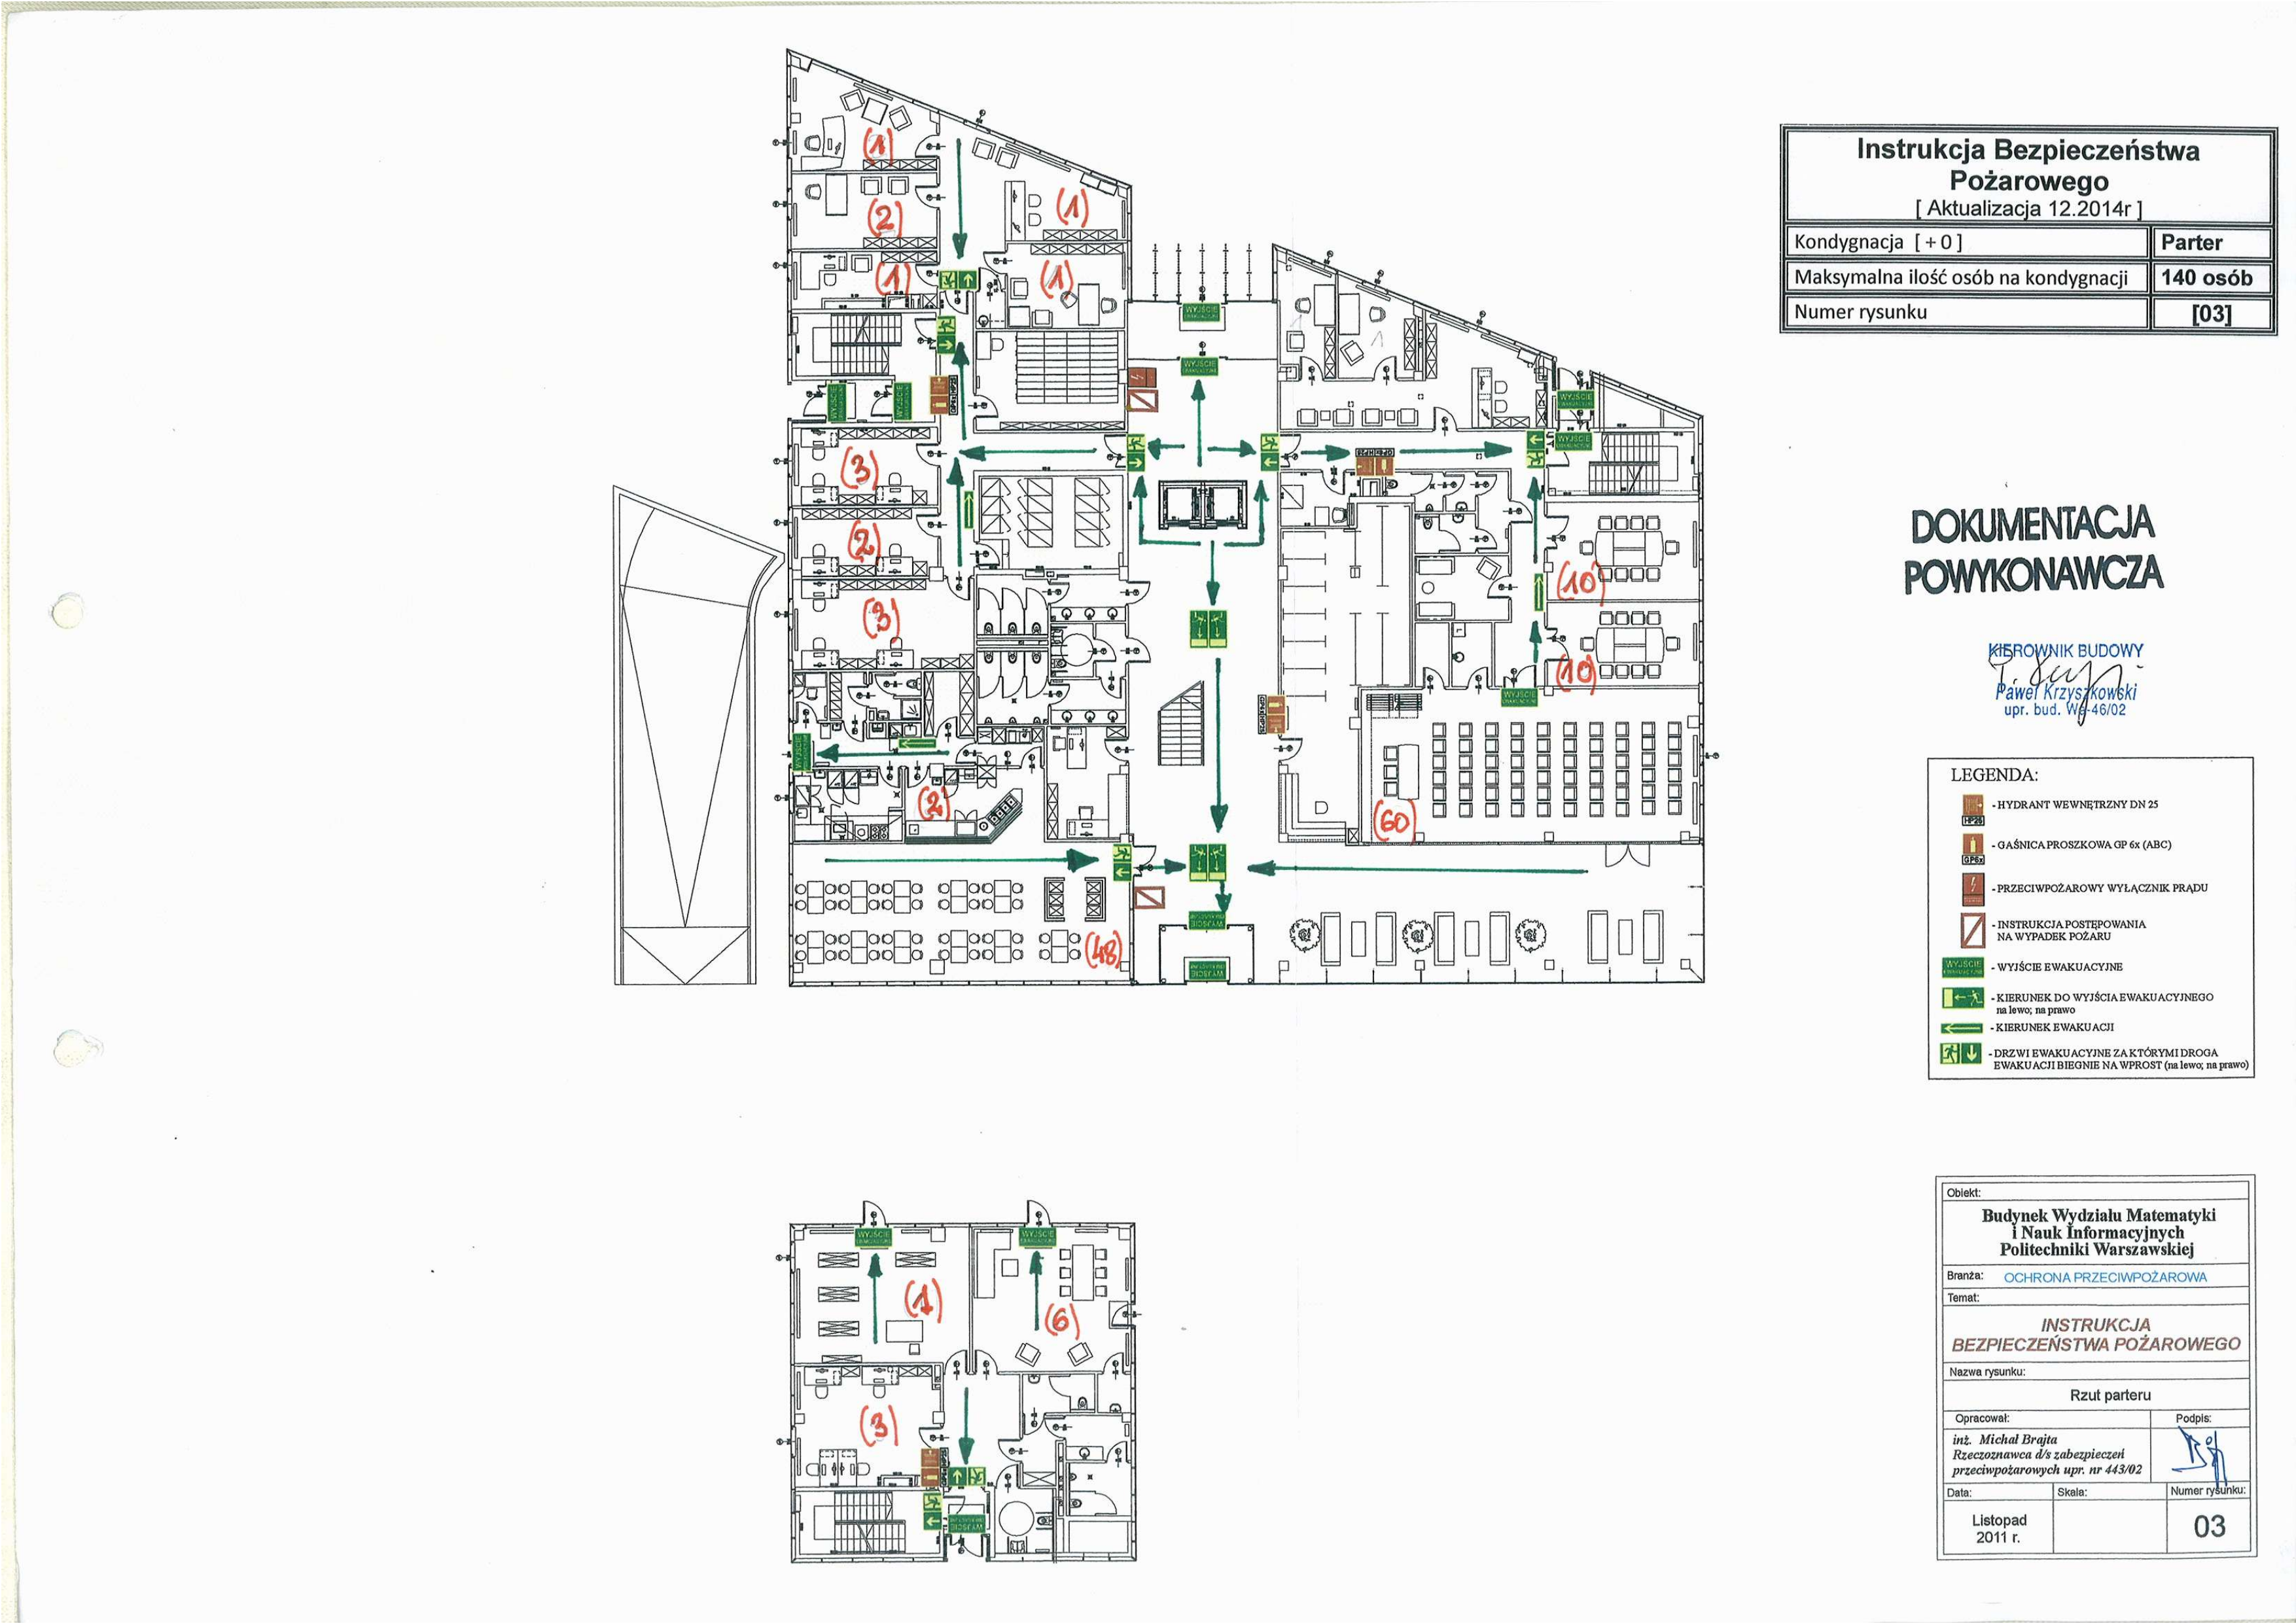
\includegraphics[width=\linewidth,height=0.22\textheight,keepaspectratio]{parter.png}
    \end{minipage}
    \hfill
    \begin{minipage}[t]{0.49\textwidth}
        \centering
        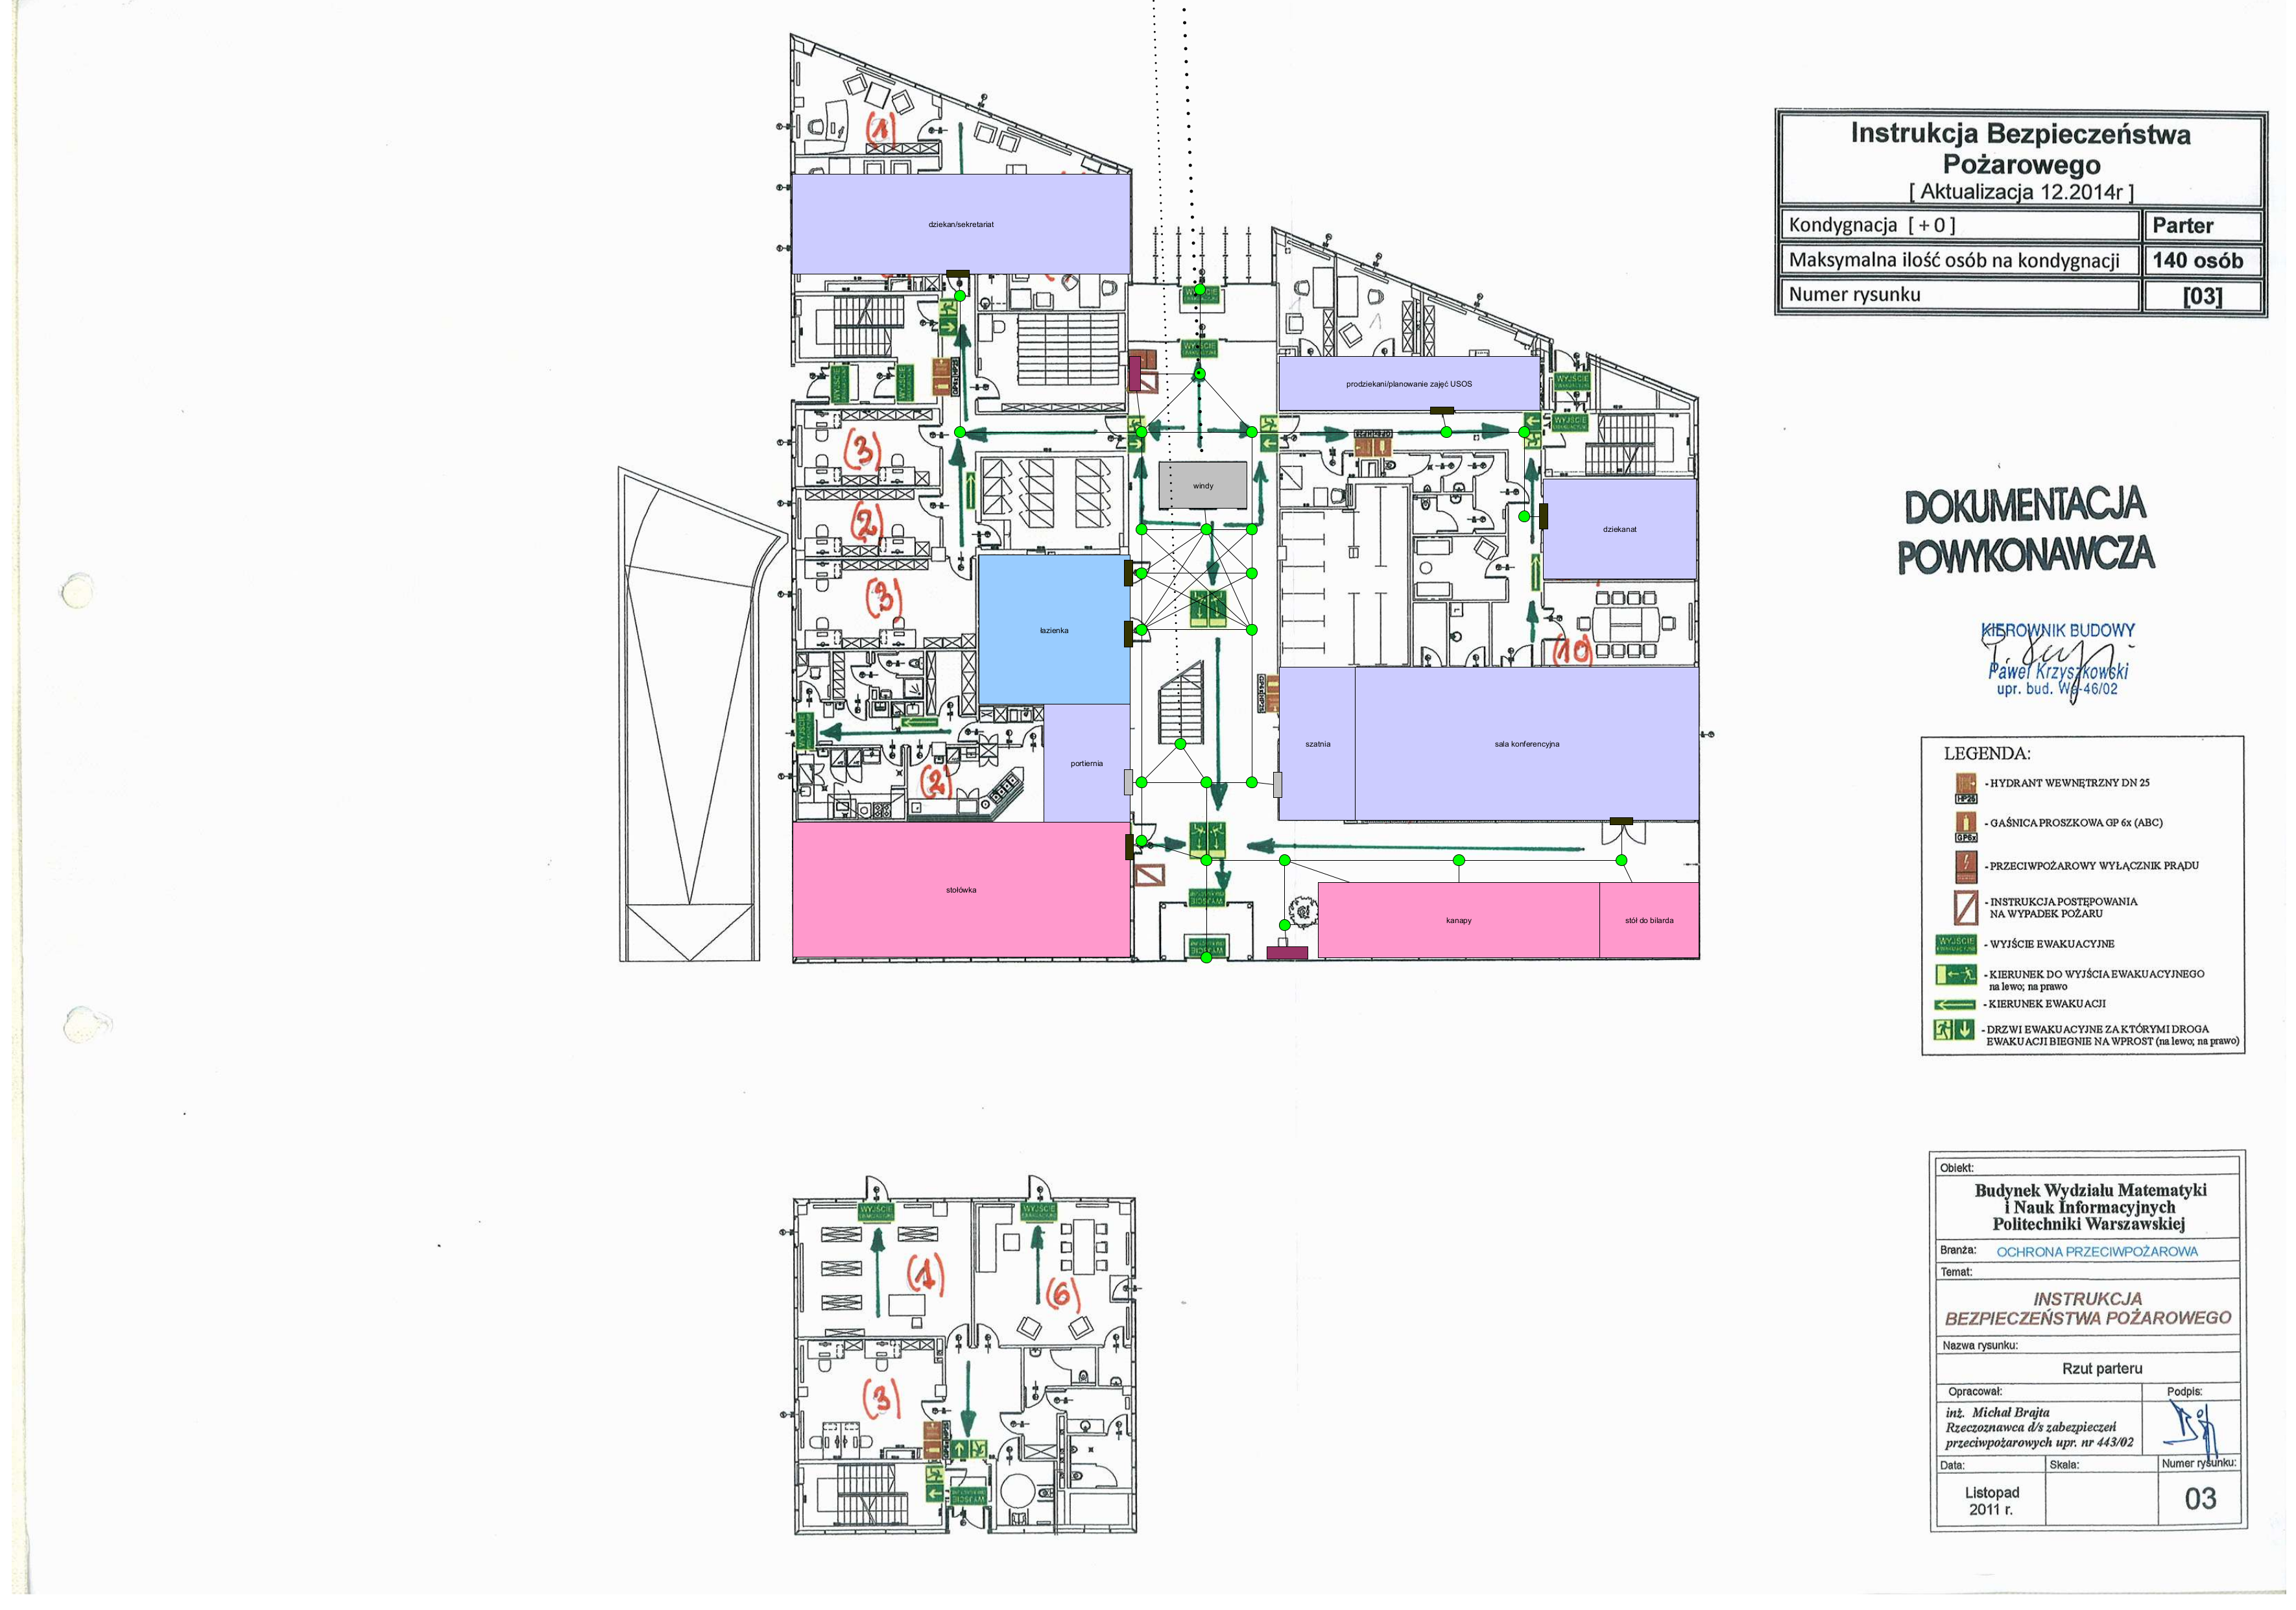
\includegraphics[width=\linewidth,height=0.22\textheight,keepaspectratio]{MINImapsGraf_6x1.png}
    \end{minipage}
    \caption{Parter: plan ewakuacyjny przed wektoryzacją (po lewej) oraz plan po wektoryzacji (po prawej).}
    \label{fig:wektoryzacja-parter}
\end{figure}

\begin{figure}[htbp]
    \centering
    \begin{minipage}[t]{0.49\textwidth}
        \centering
        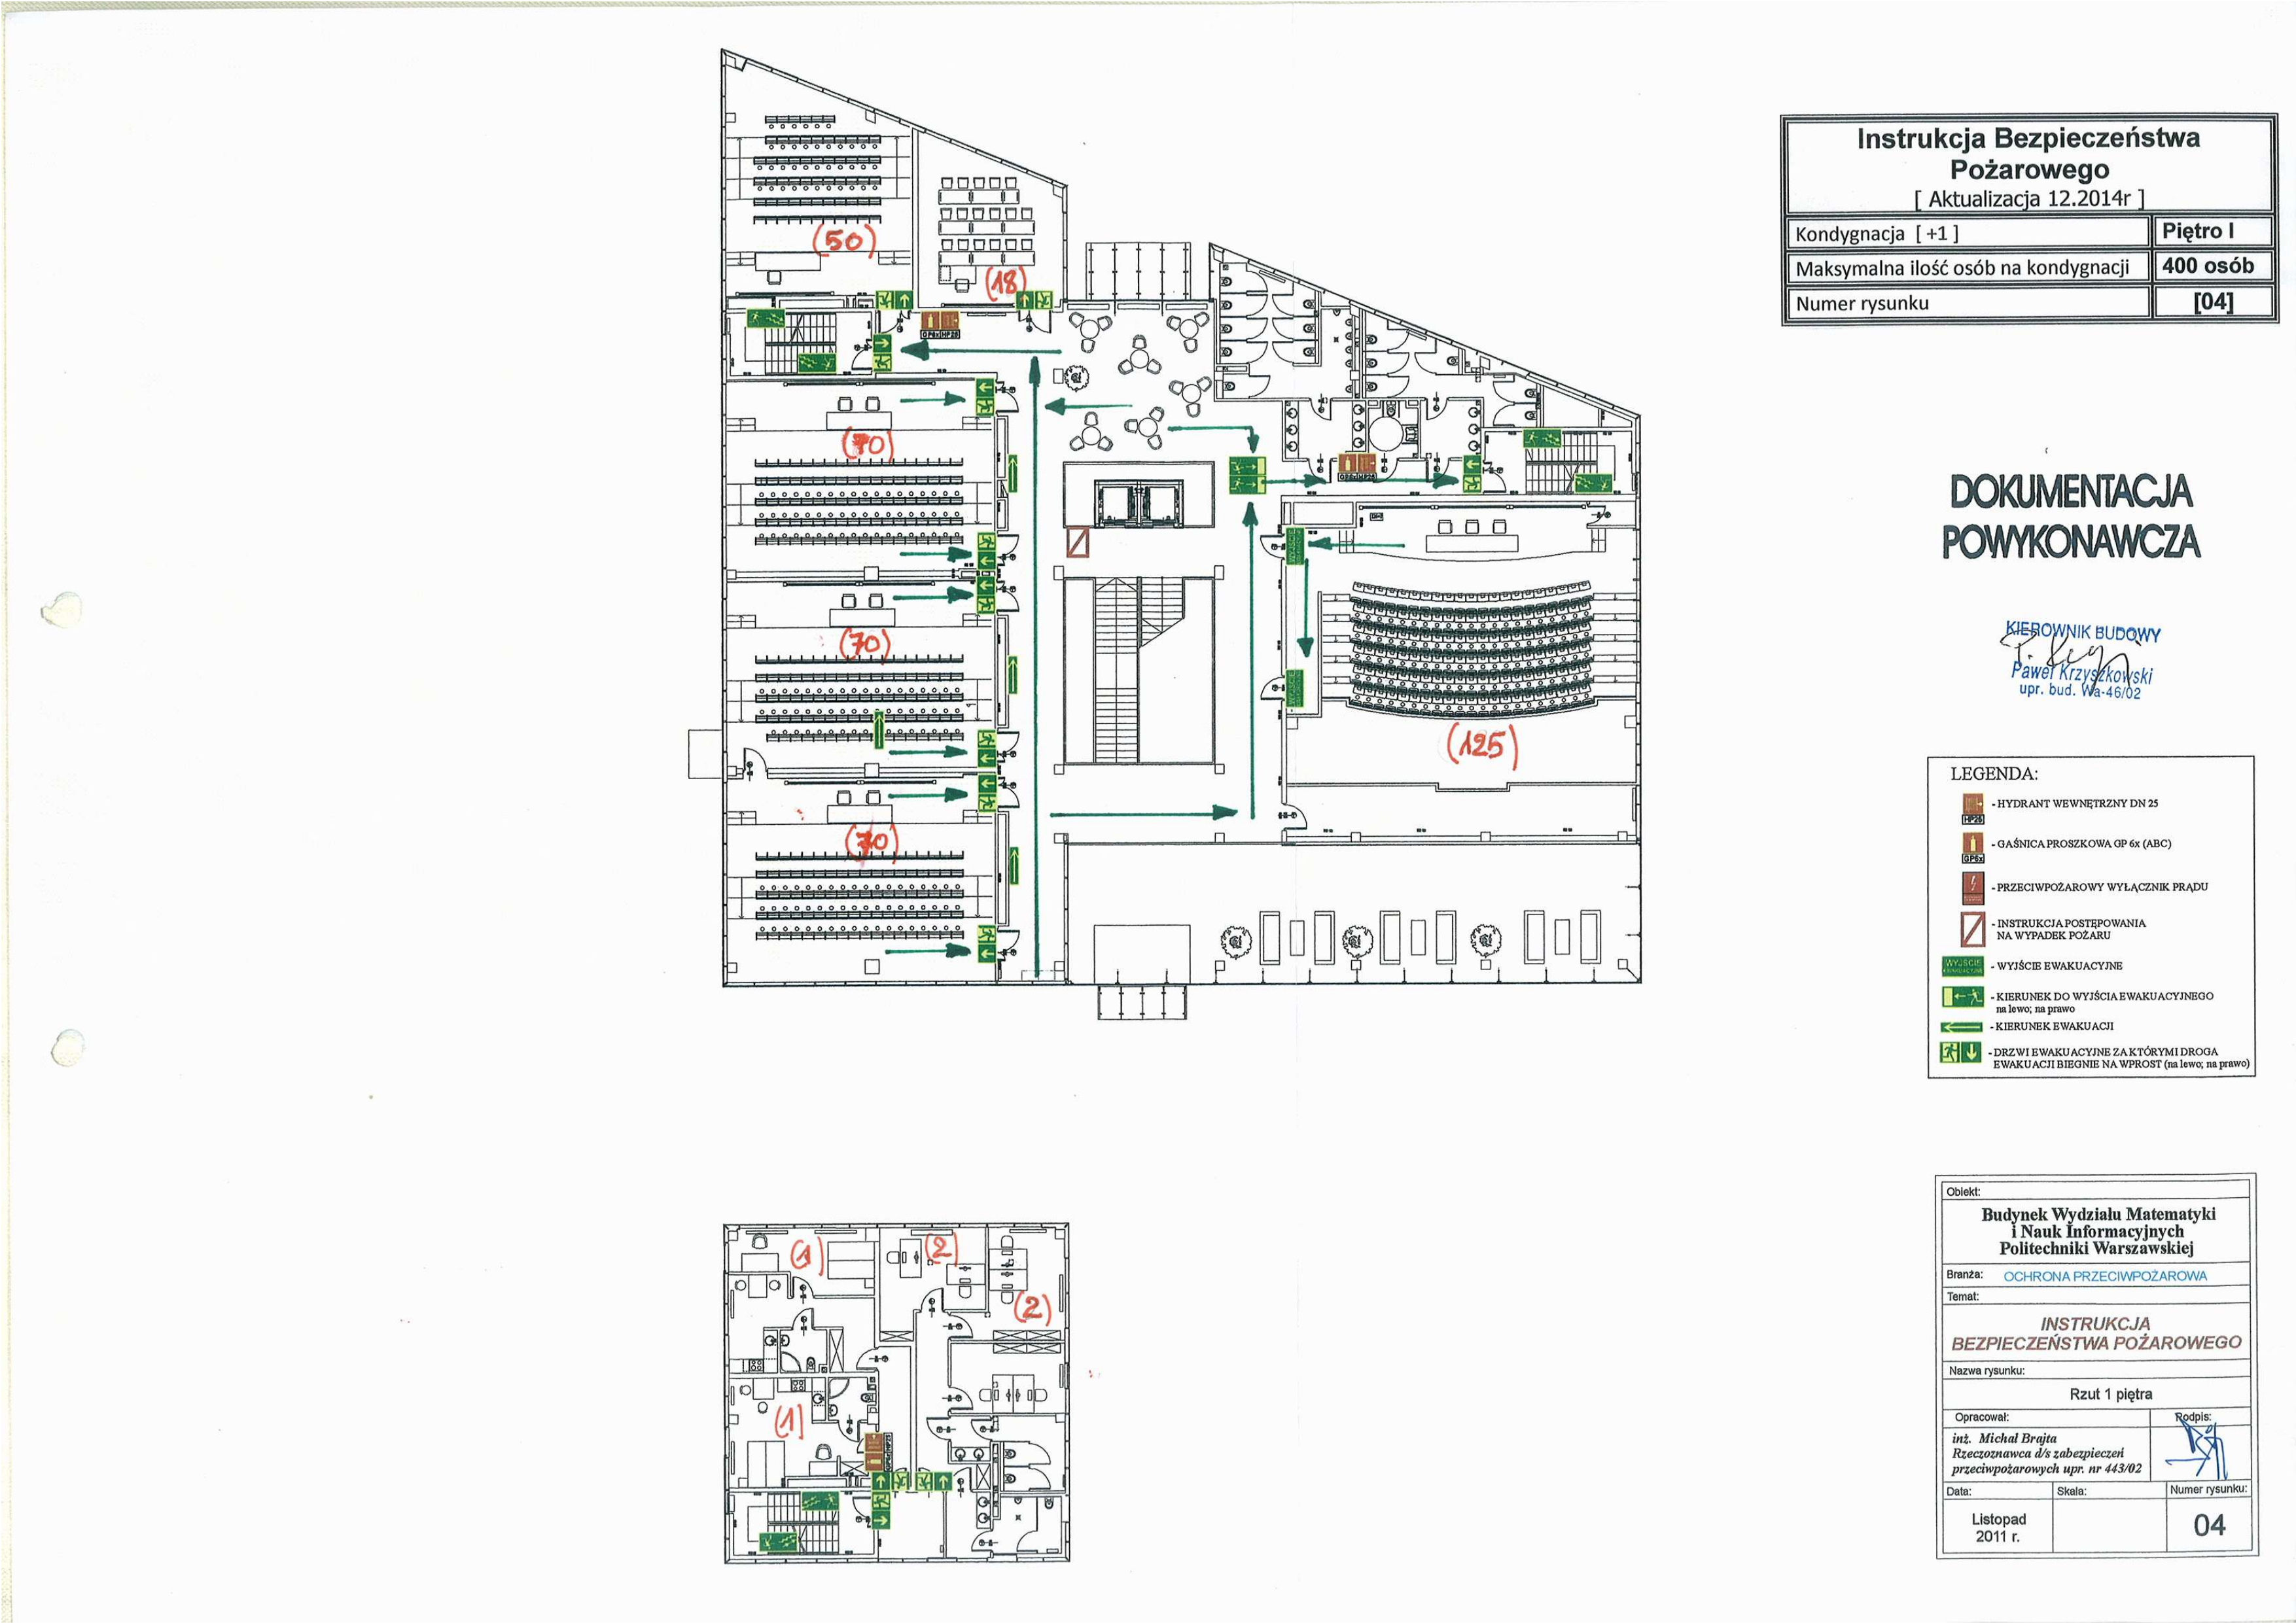
\includegraphics[width=\linewidth,height=0.22\textheight,keepaspectratio]{1pietro.png}
    \end{minipage}
    \hfill
    \begin{minipage}[t]{0.49\textwidth}
        \centering
        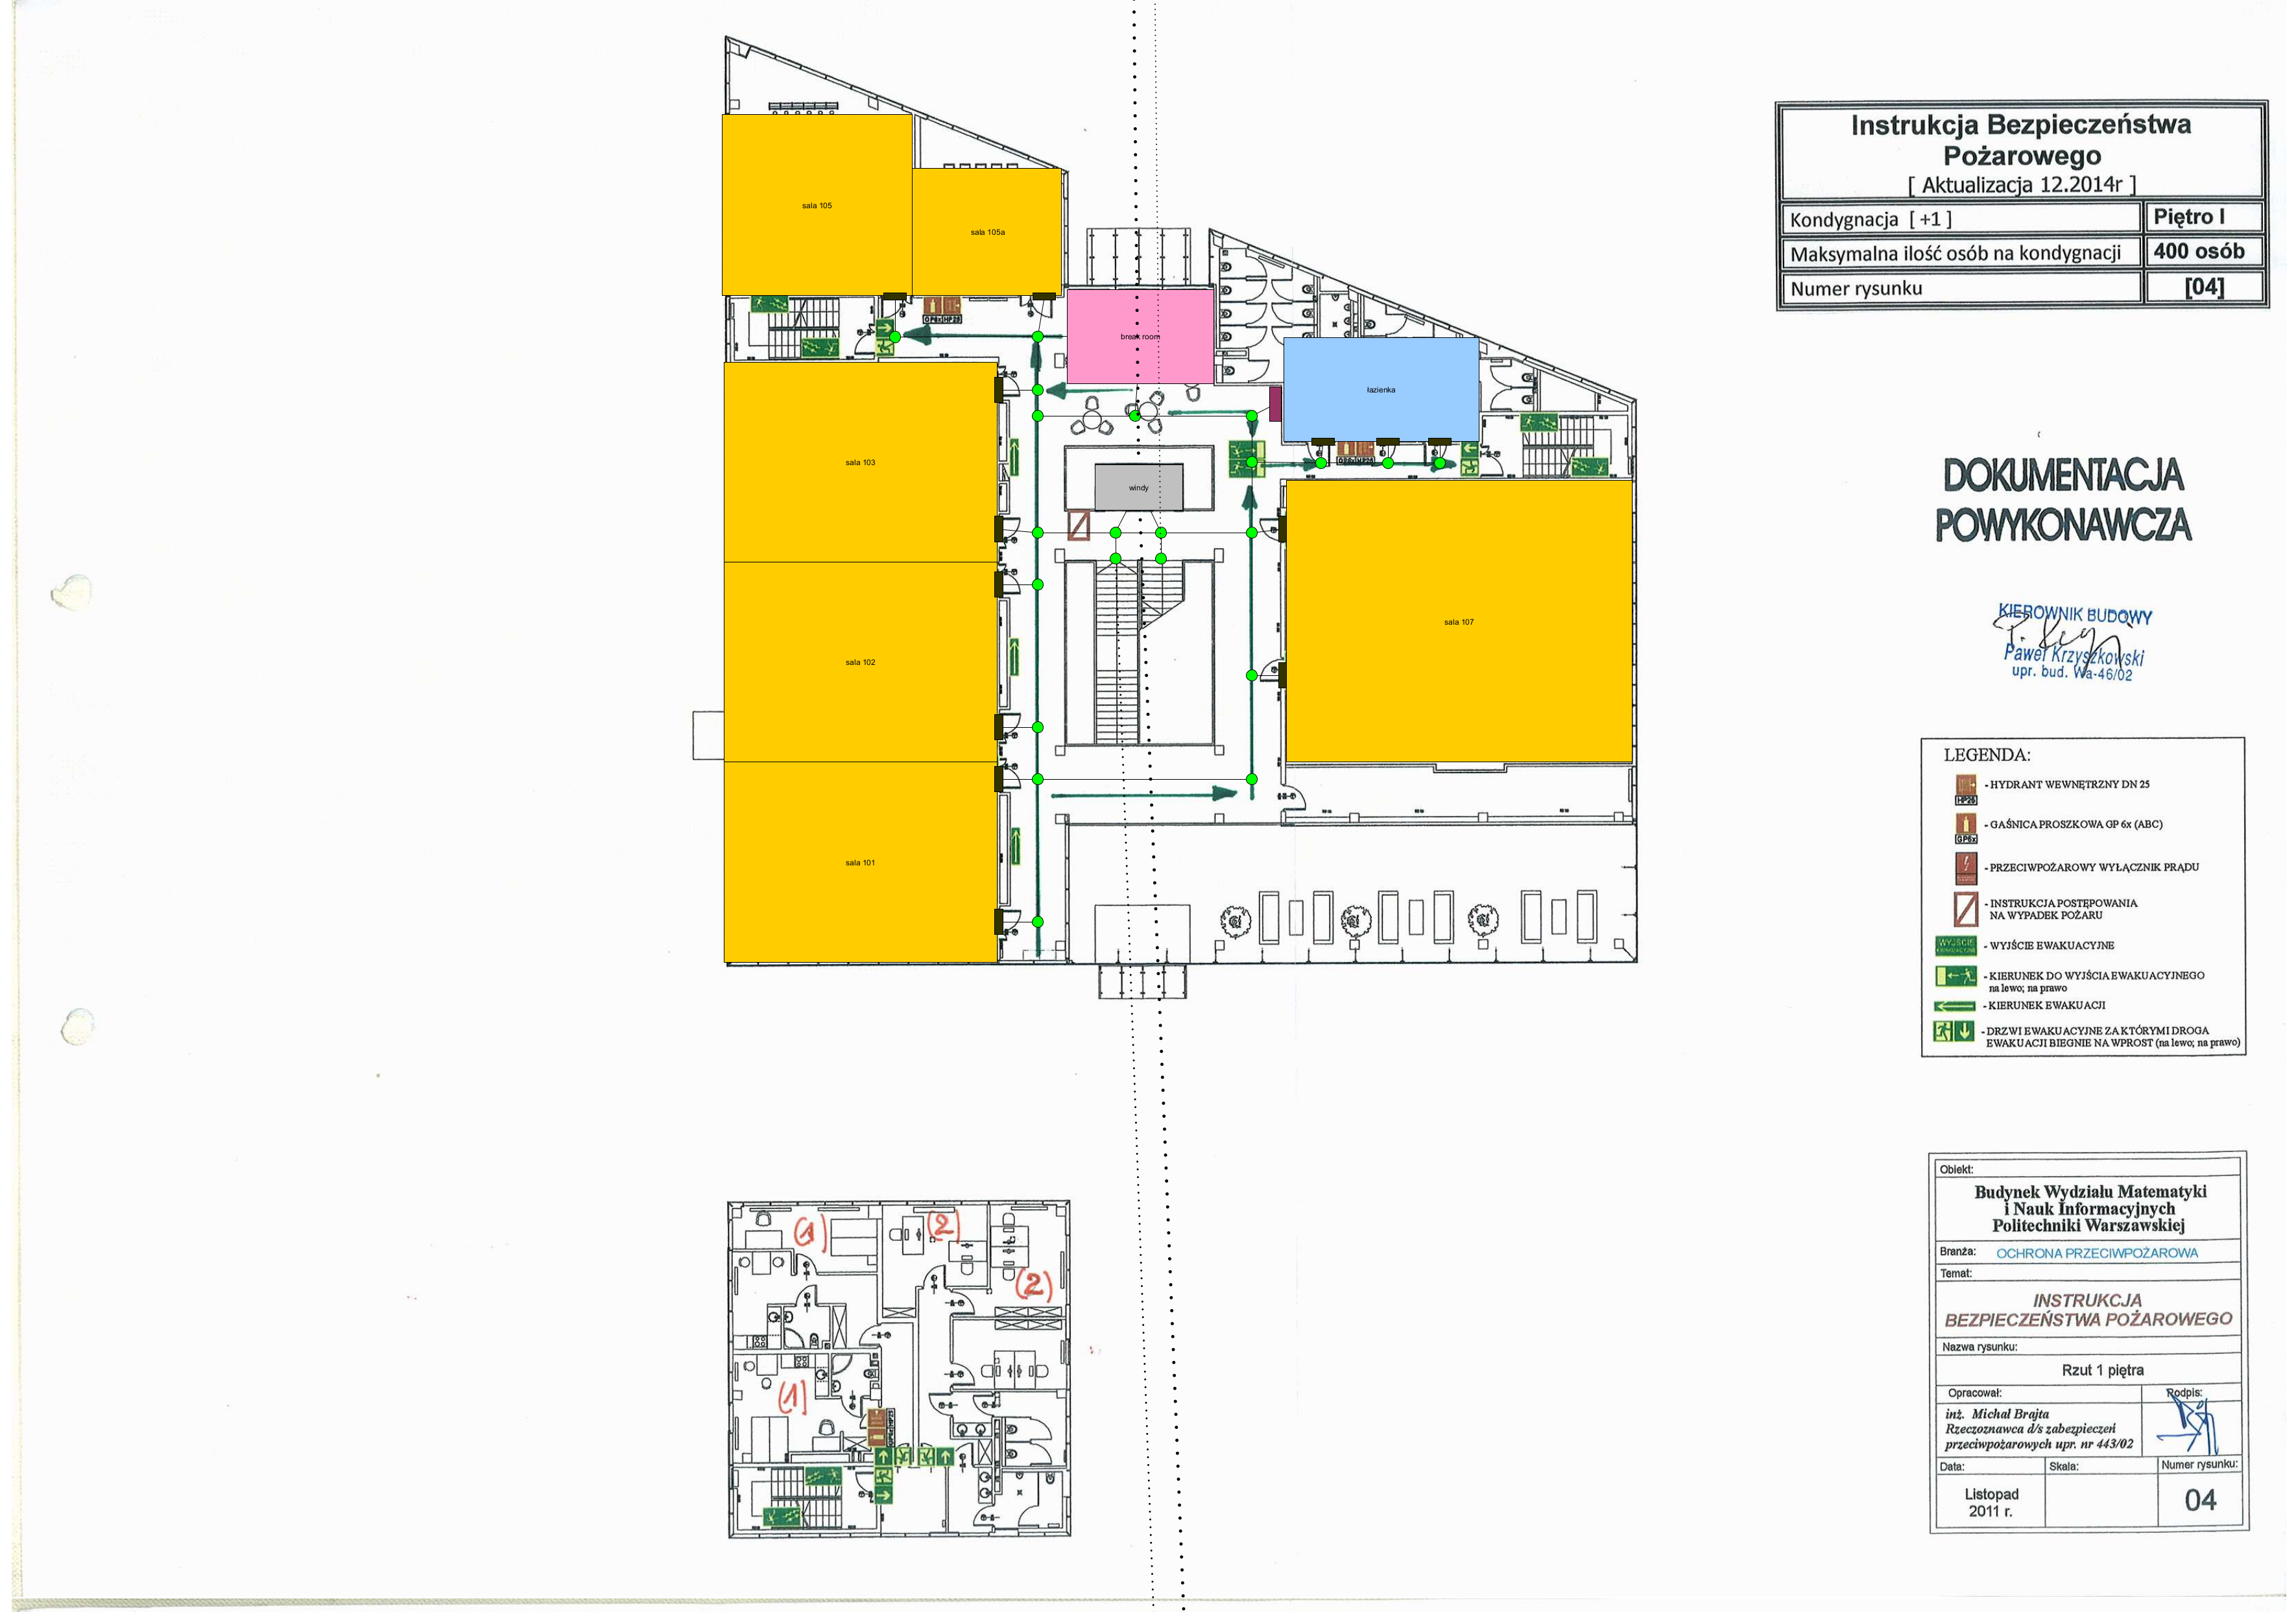
\includegraphics[width=\linewidth,height=0.22\textheight,keepaspectratio]{MINImapsGraf_5x1.png}
    \end{minipage}
    \caption{Piętro 1: plan ewakuacyjny przed wektoryzacją (po lewej) oraz plan po wektoryzacji (po prawej).}
    \label{fig:wektoryzacja-p1}
\end{figure}
\clearpage

\begin{figure}[t]
    \centering
    \begin{minipage}[t]{0.49\textwidth}
        \centering
        \includegraphics[width=\linewidth,height=0.22\textheight,keepaspectratio]{2pietro.png}
    \end{minipage}
    \hfill
    \begin{minipage}[t]{0.49\textwidth}
        \centering
        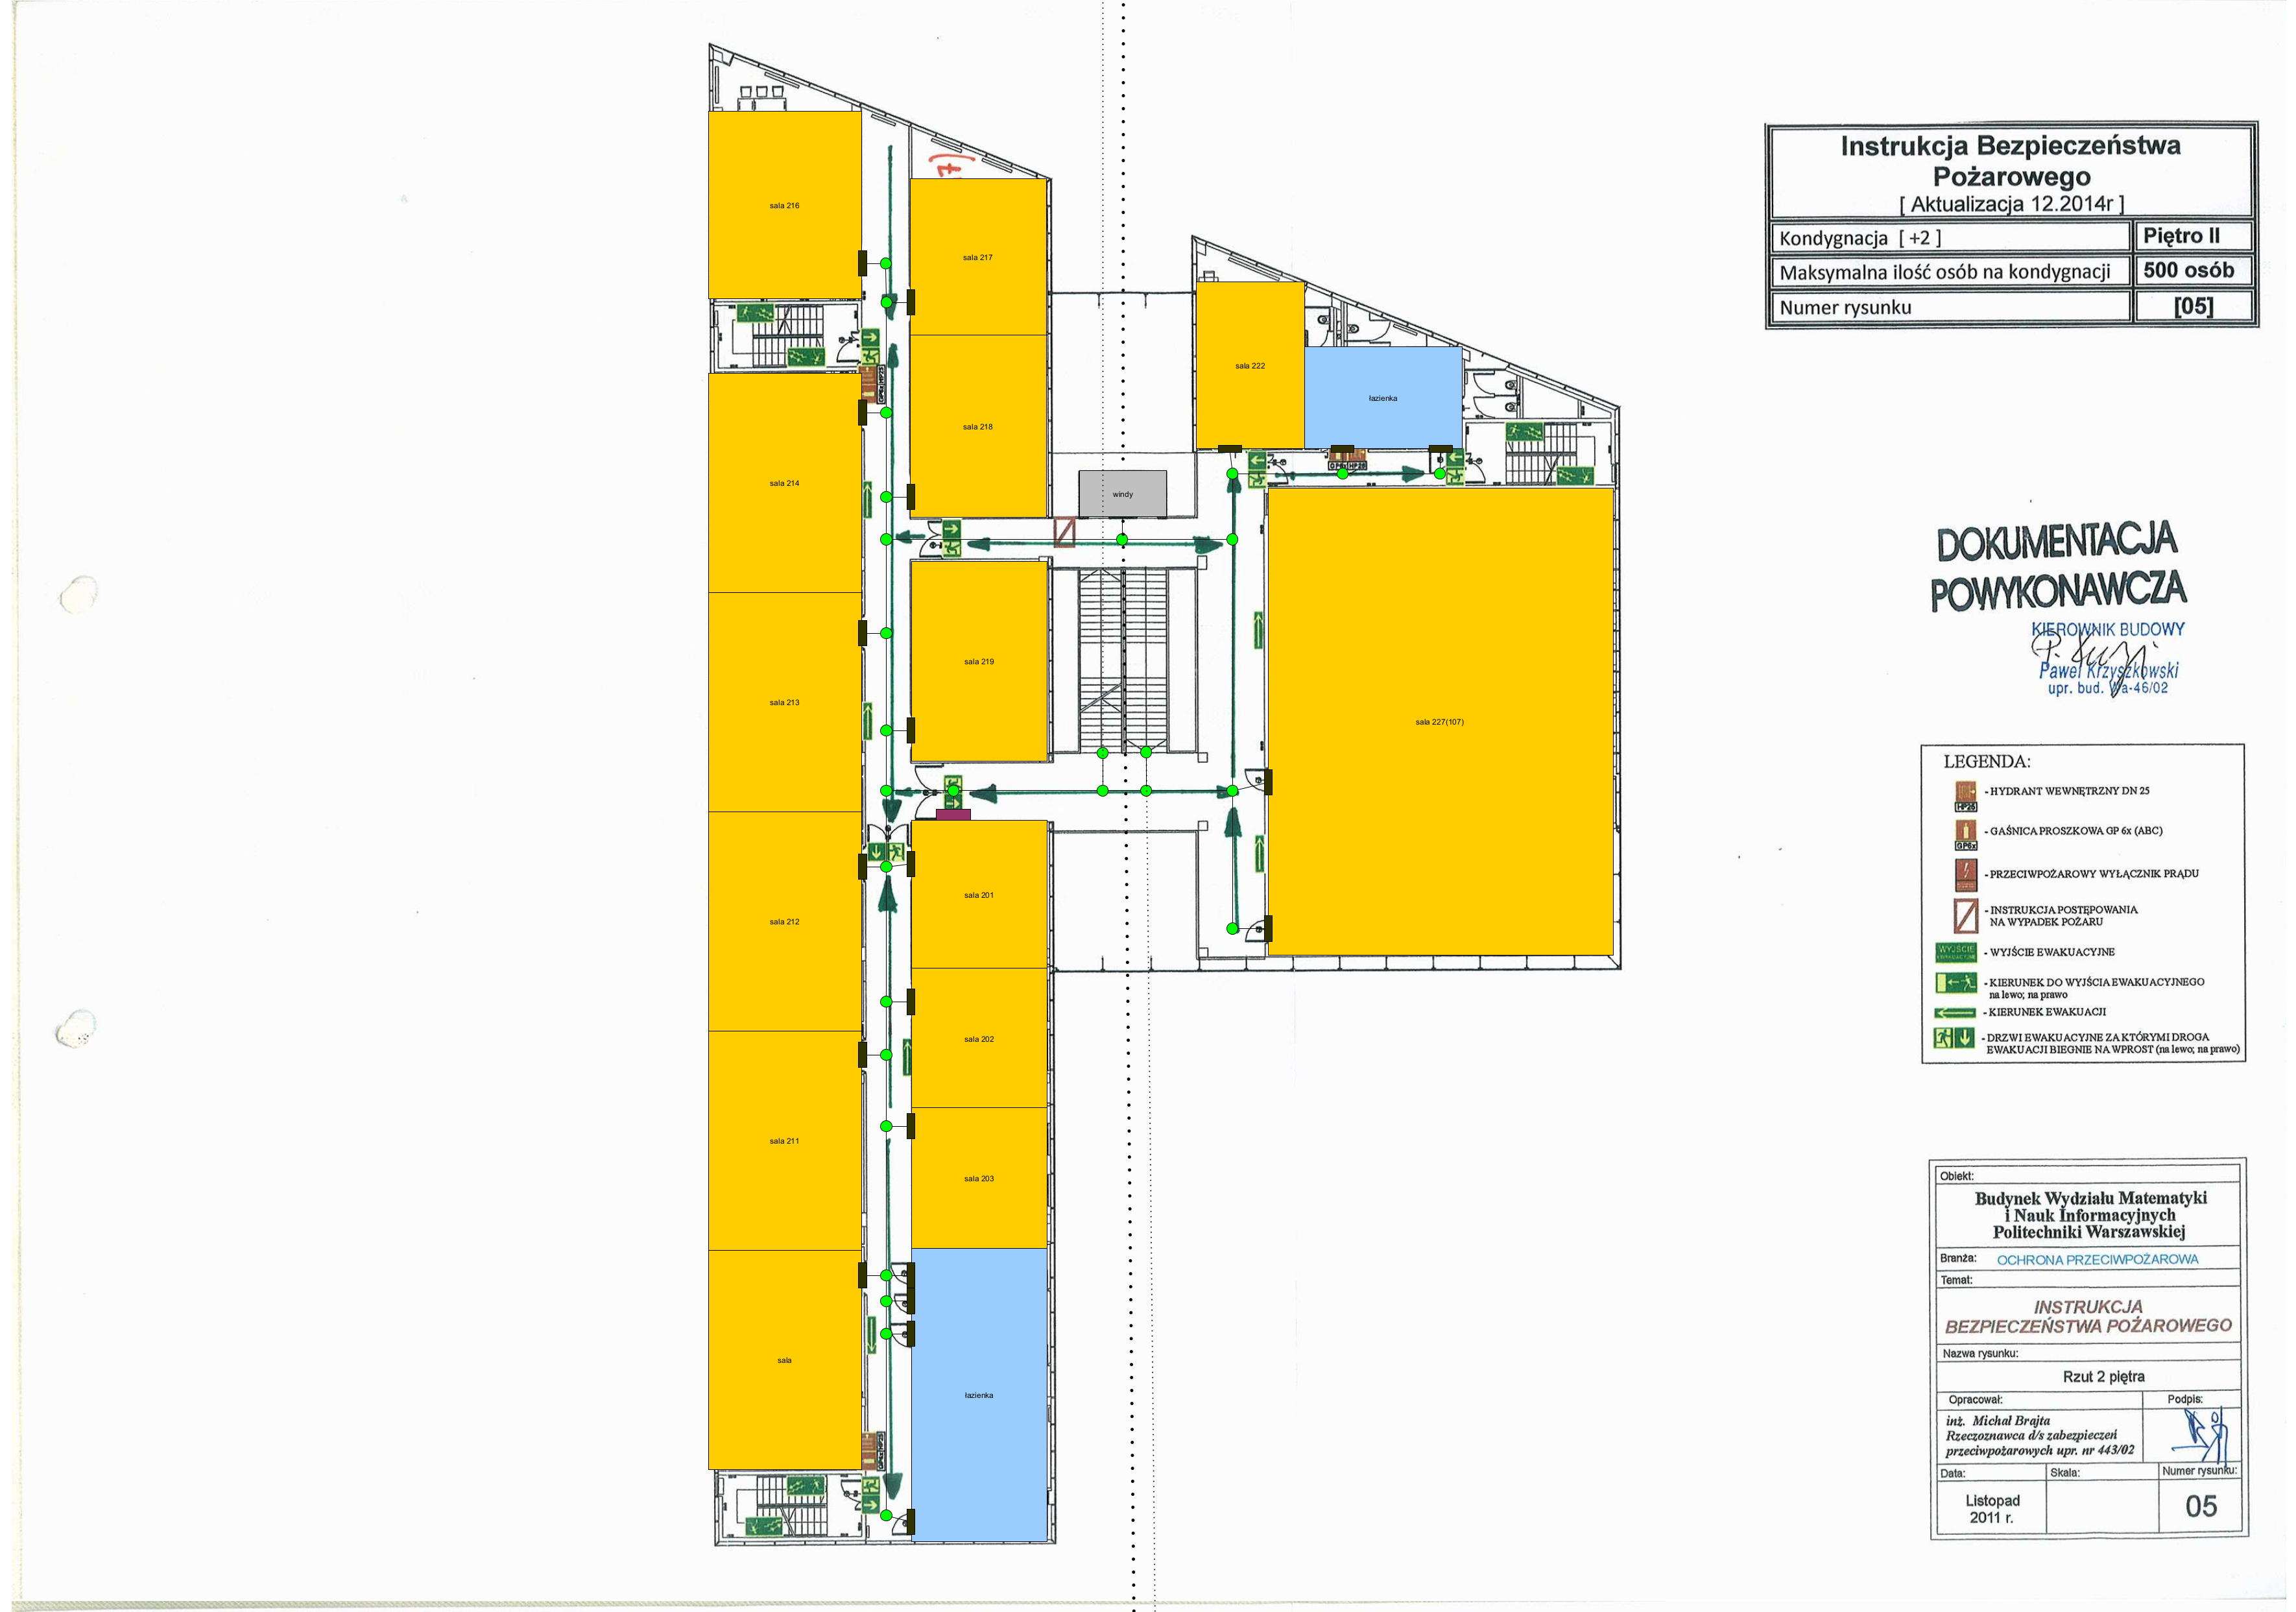
\includegraphics[width=\linewidth,height=0.22\textheight,keepaspectratio]{MINImapsGraf_4x1.png}
    \end{minipage}
    \caption{Piętro 2: plan ewakuacyjny przed wektoryzacją (po lewej) oraz plan po wektoryzacji (po prawej).}
    \label{fig:wektoryzacja-p2}
\end{figure}

\begin{figure}[t]
    \centering
    \begin{minipage}[t]{0.49\textwidth}
        \centering
        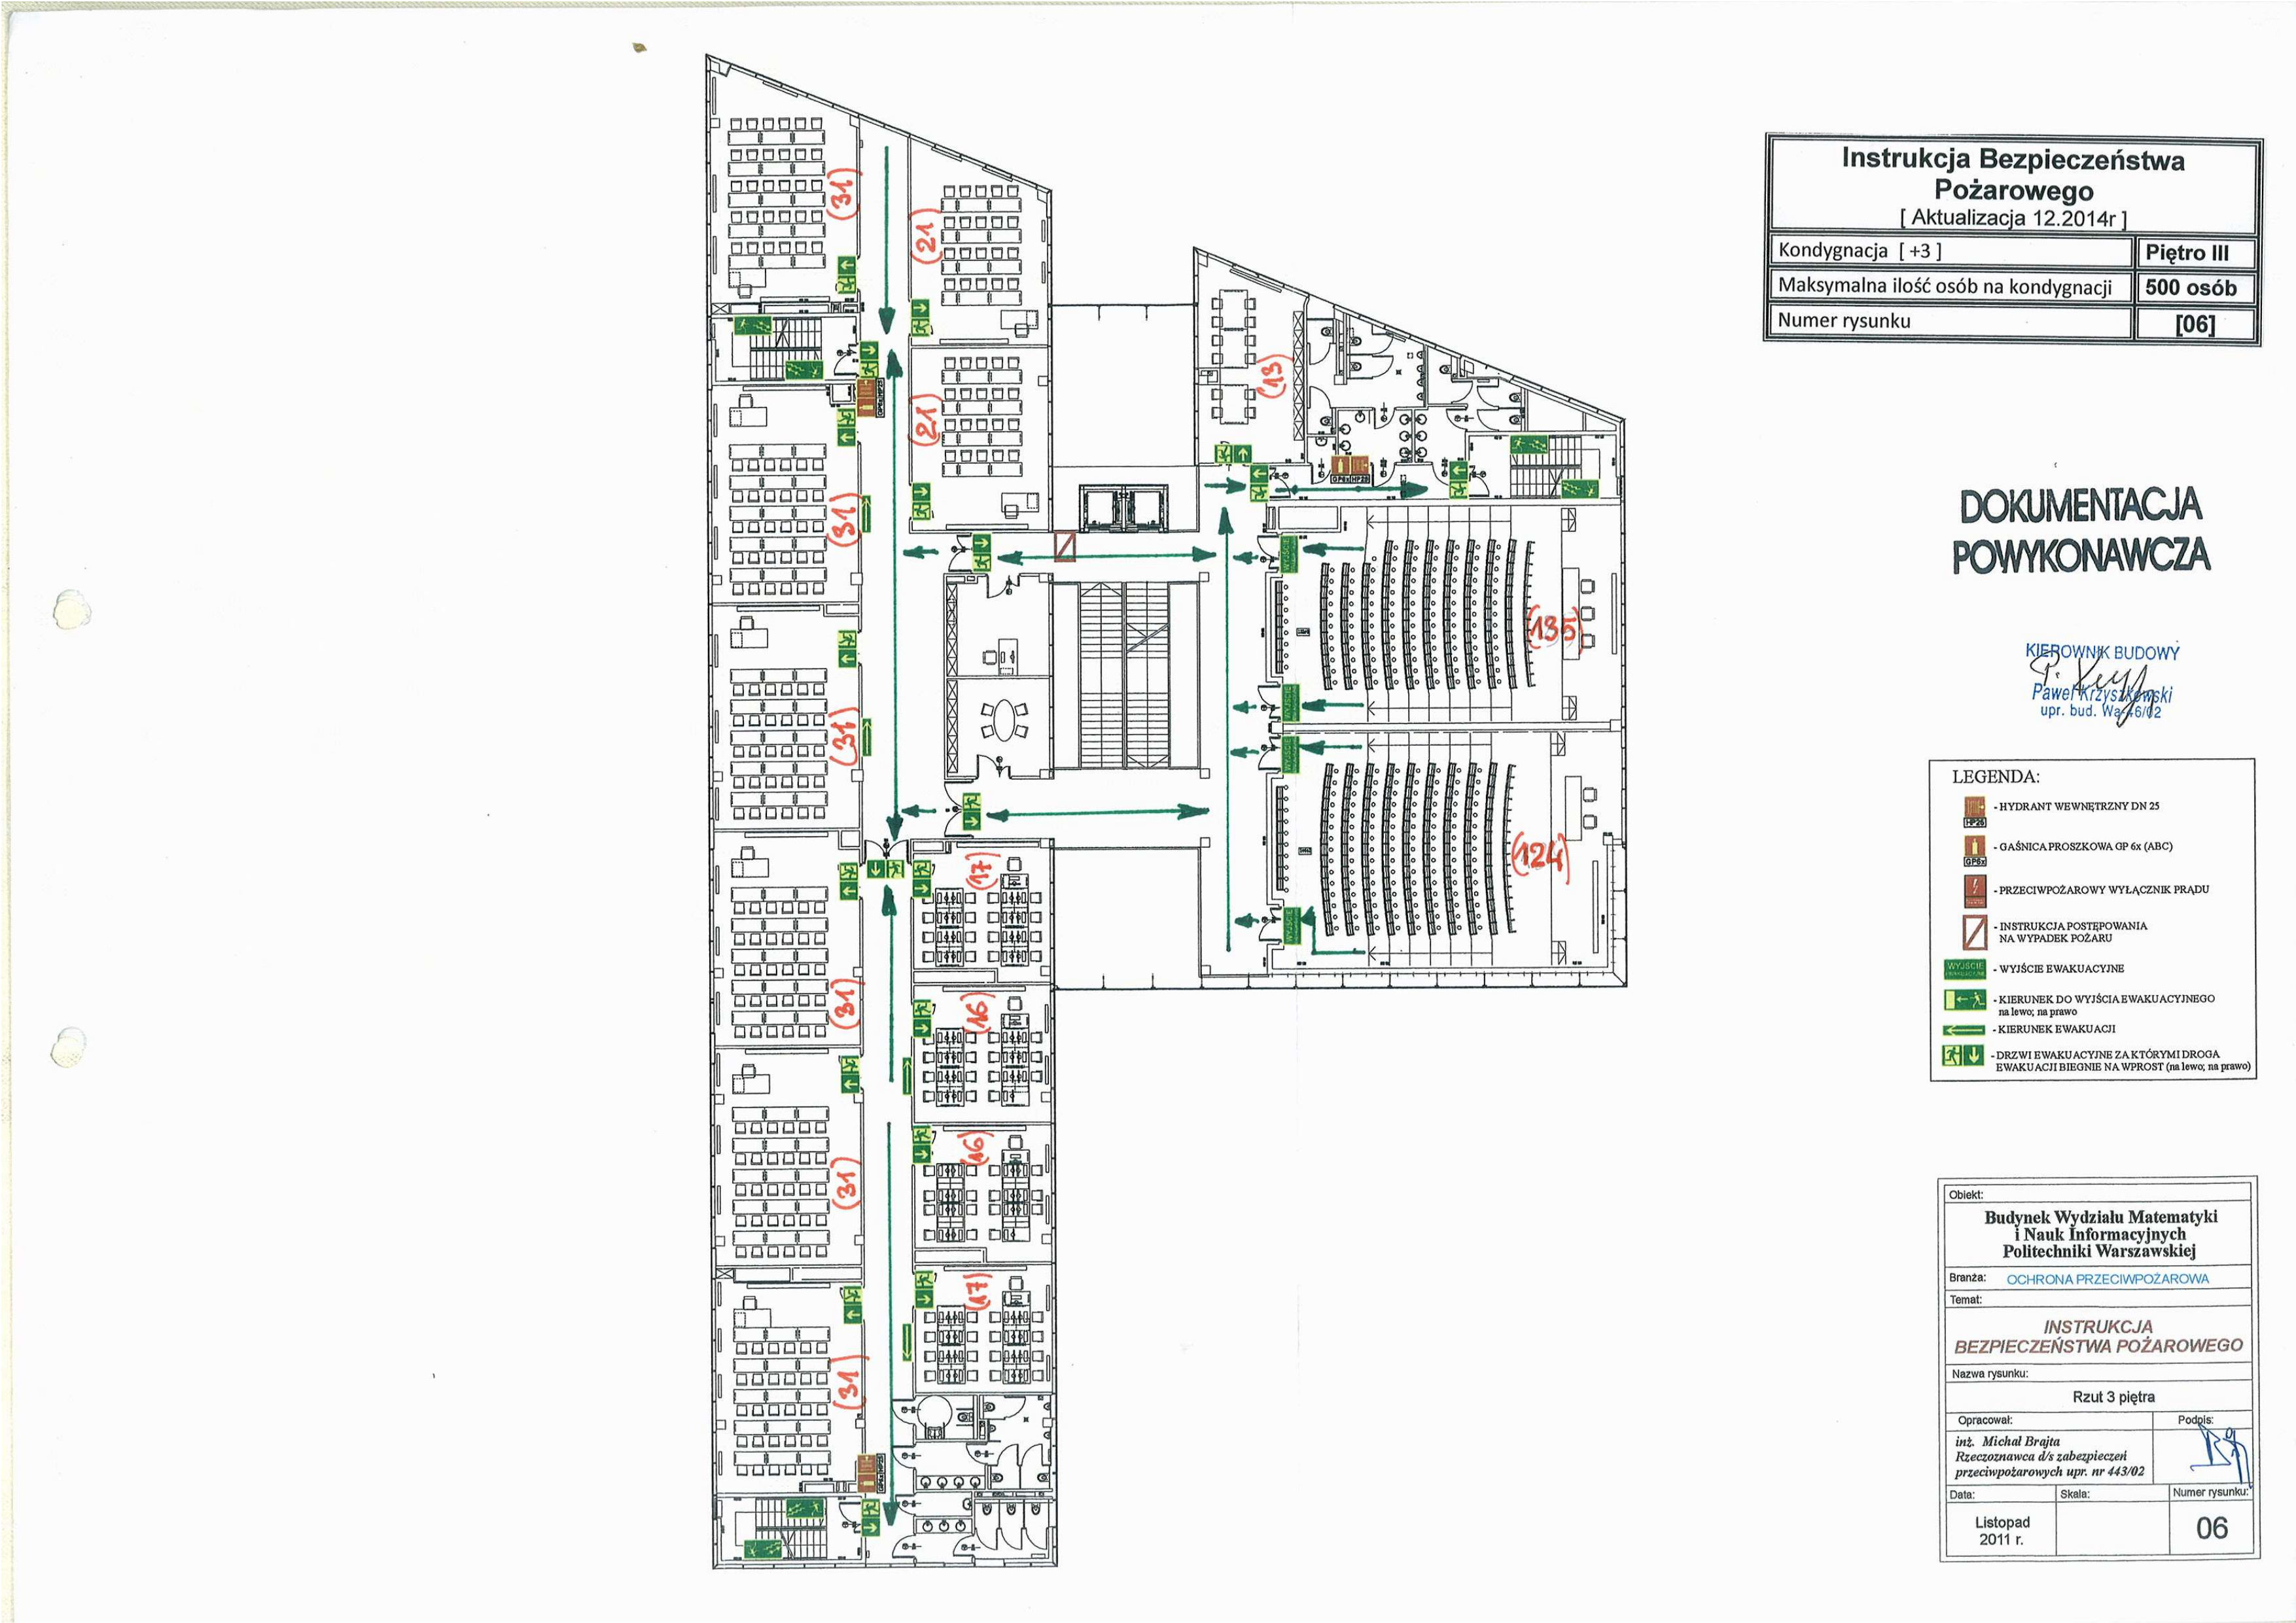
\includegraphics[width=\linewidth,height=0.22\textheight,keepaspectratio]{3pietro.png}
    \end{minipage}
    \hfill
    \begin{minipage}[t]{0.49\textwidth}
        \centering
        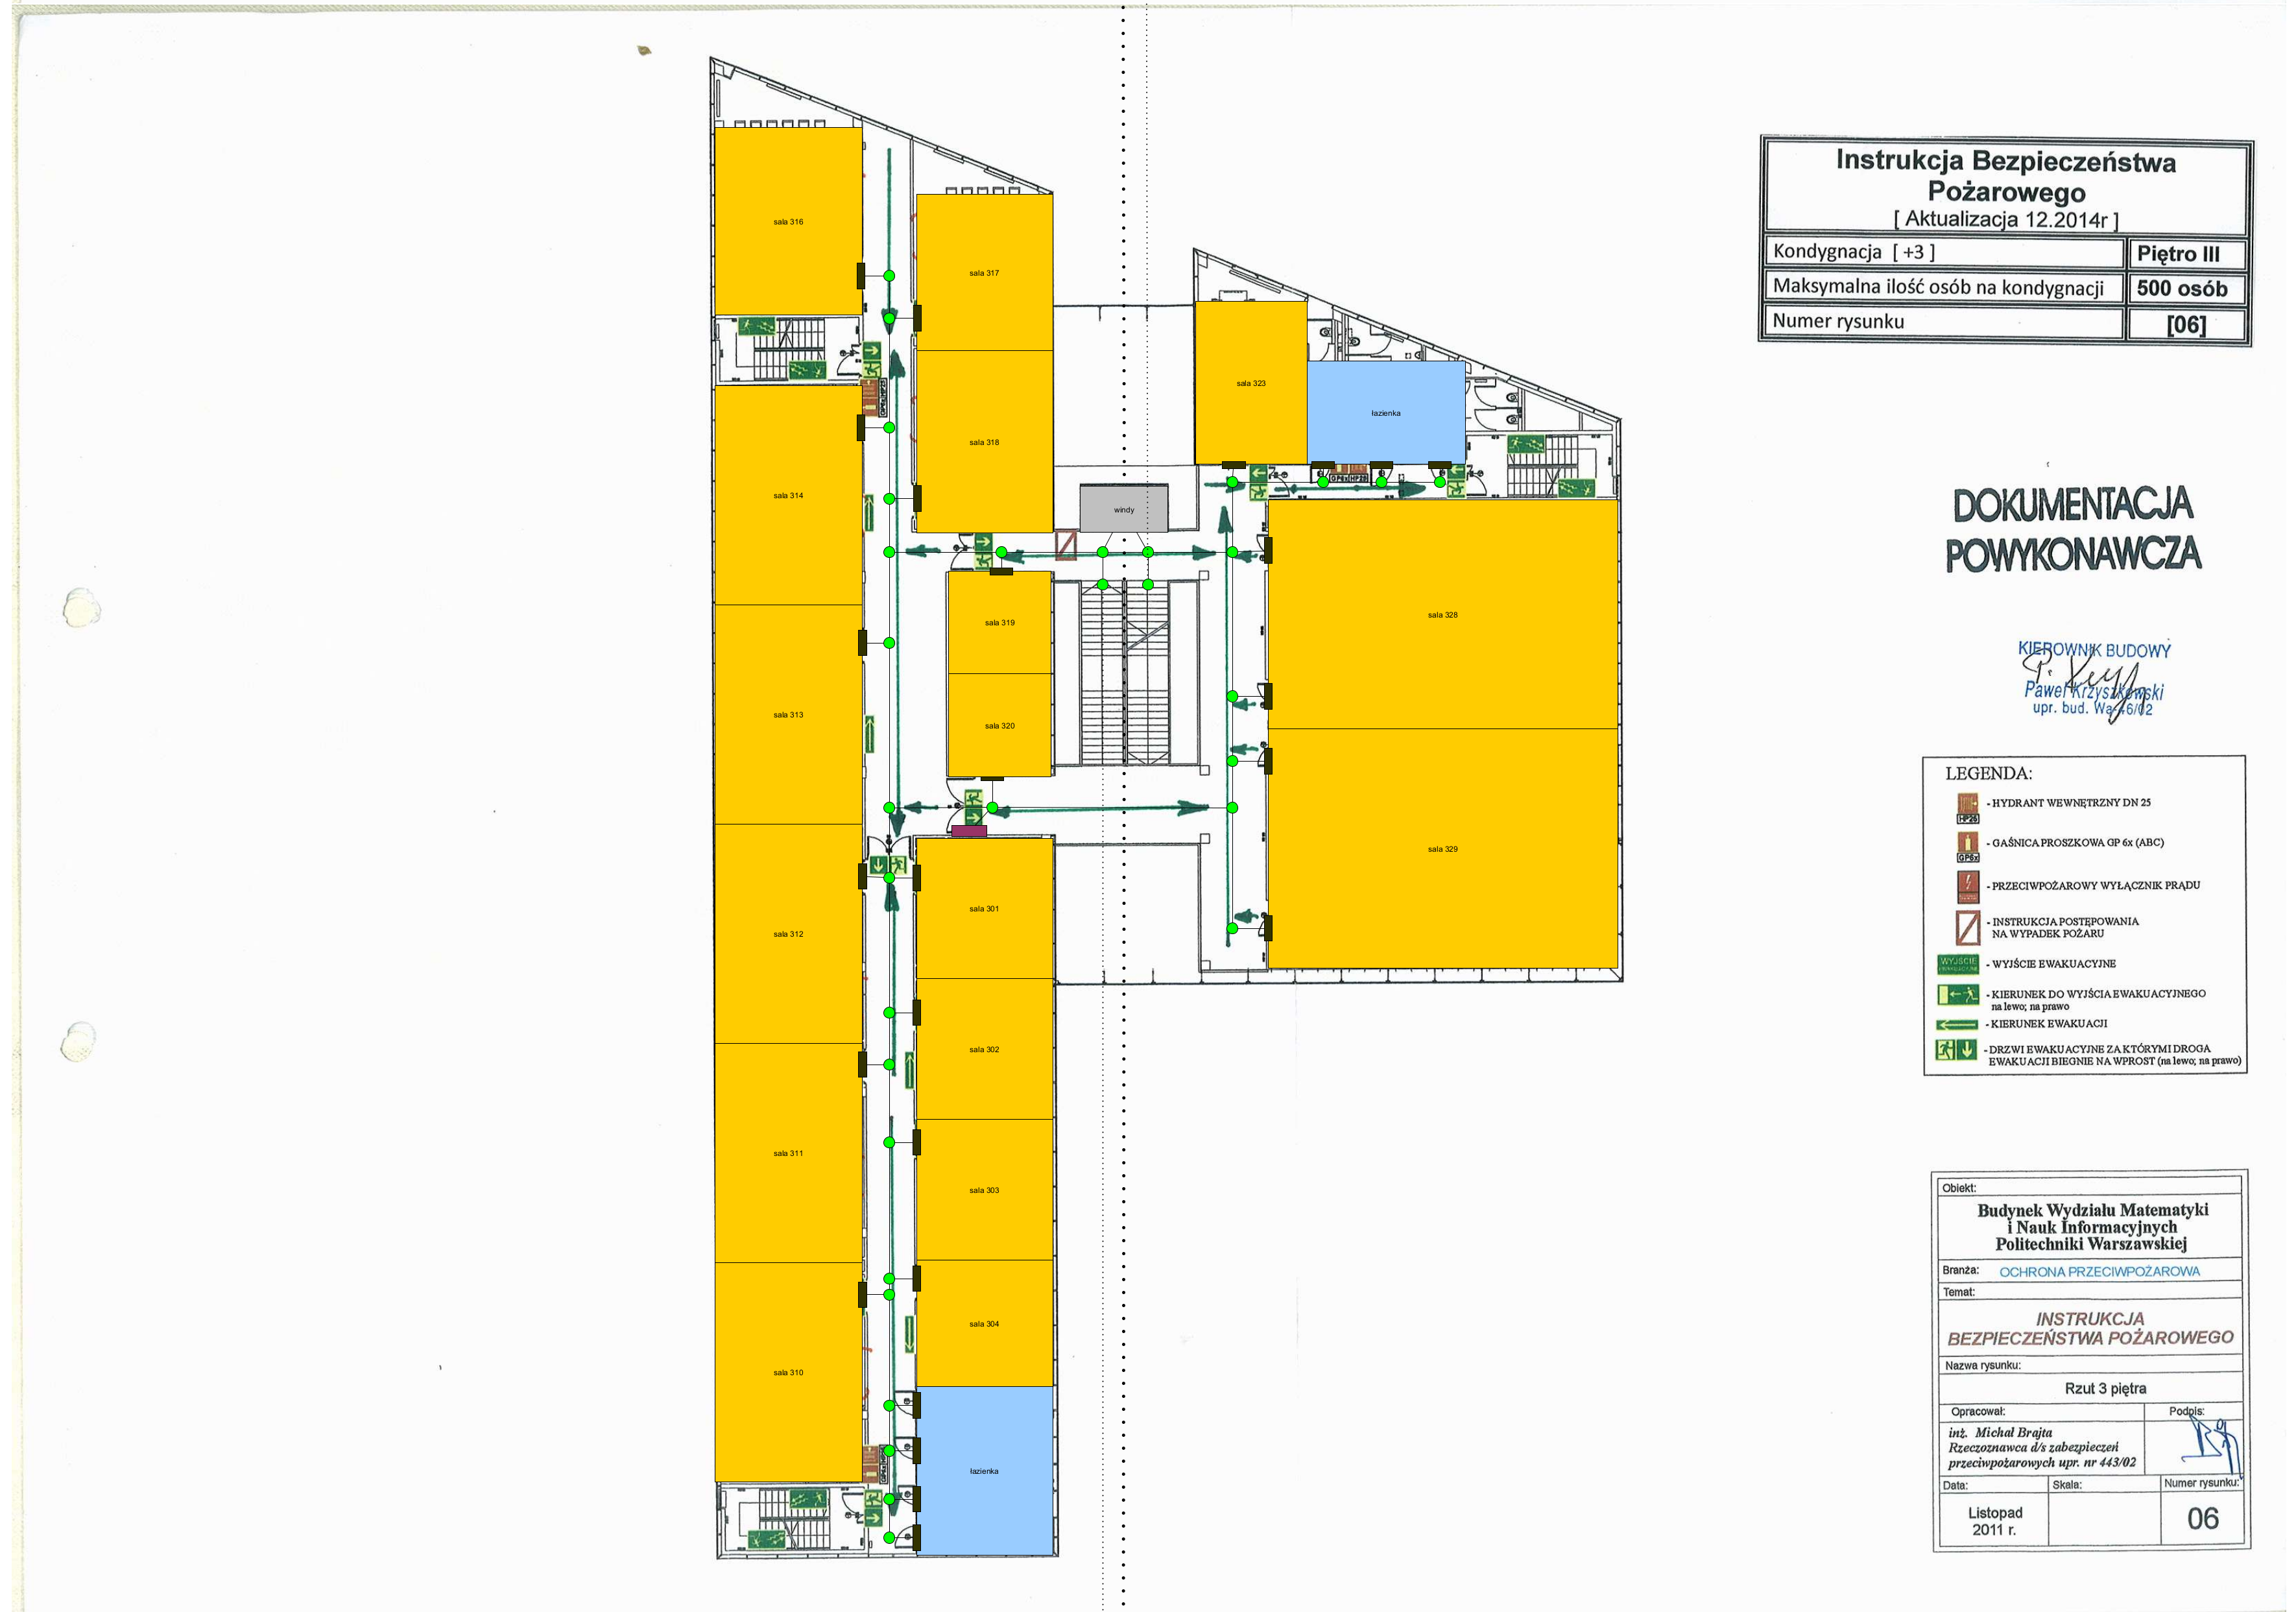
\includegraphics[width=\linewidth,height=0.22\textheight,keepaspectratio]{MINImapsGraf_3x1.png}
    \end{minipage}
    \caption{Piętro 3: plan ewakuacyjny przed wektoryzacją (po lewej) oraz plan po wektoryzacji (po prawej).}
    \label{fig:wektoryzacja-p3}
\end{figure}
\clearpage

\begin{figure}[t]
    \centering
    \begin{minipage}[t]{0.49\textwidth}
        \centering
        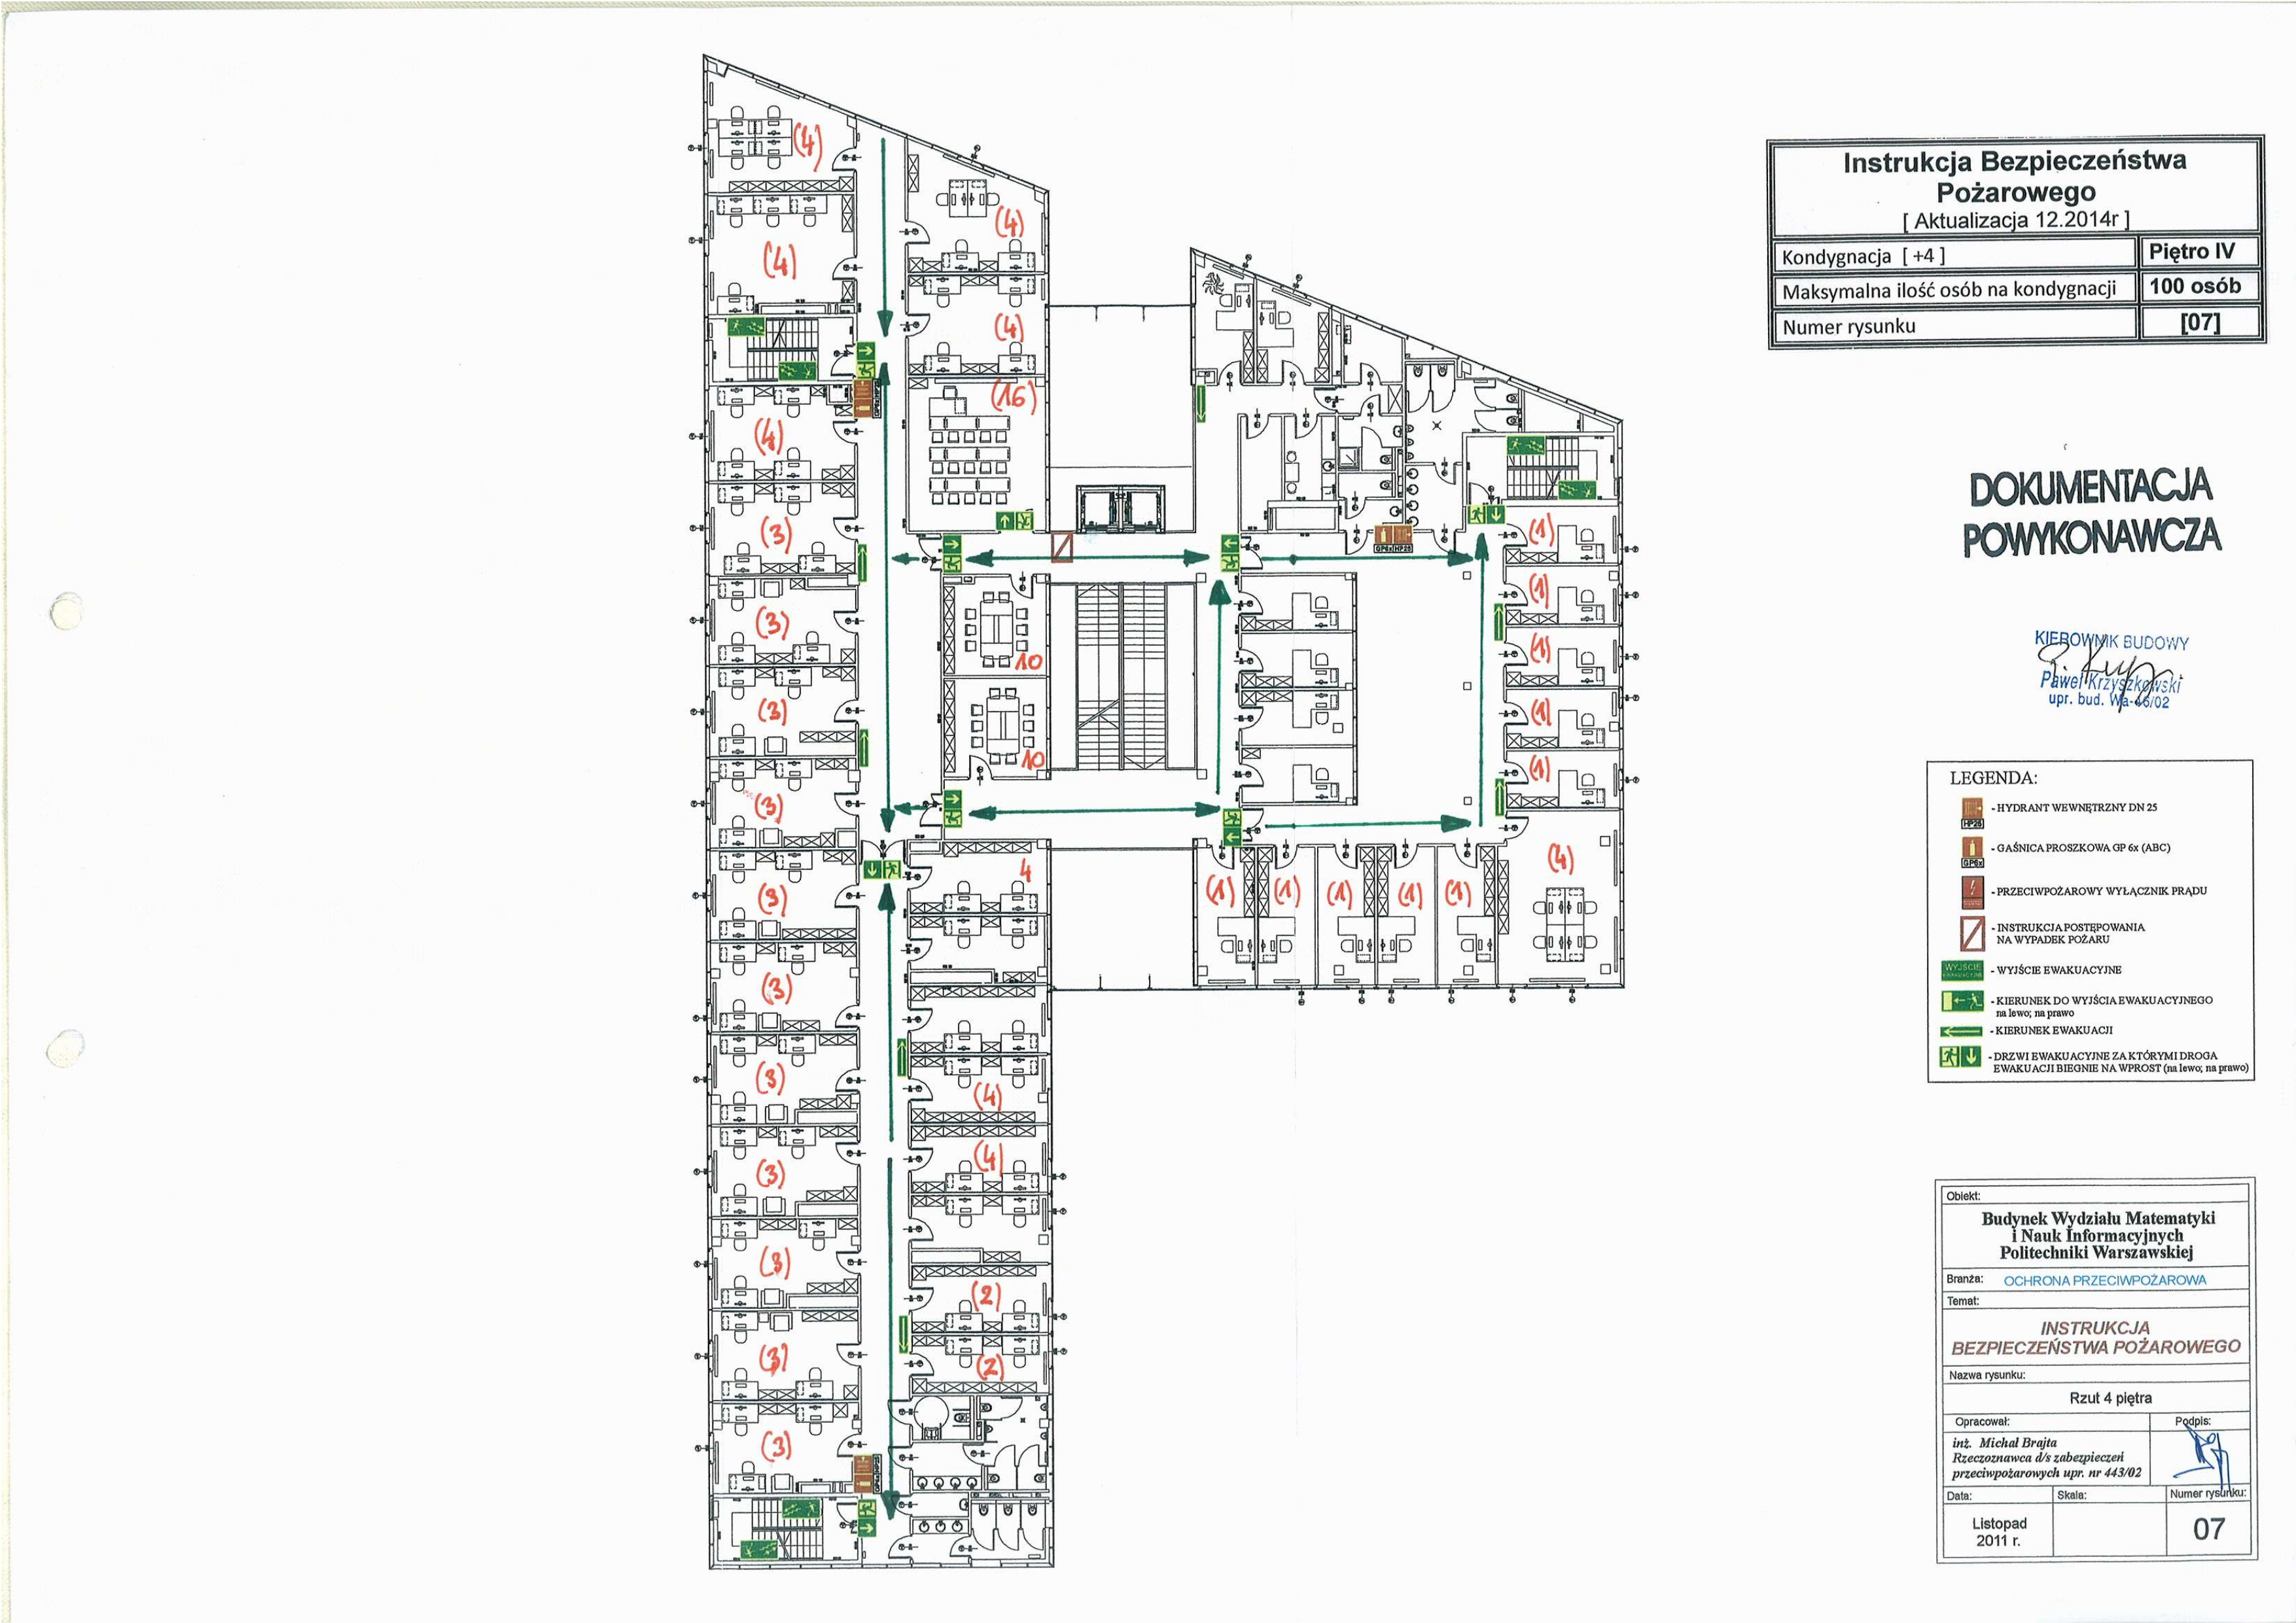
\includegraphics[width=\linewidth,height=0.22\textheight,keepaspectratio]{4pietro.png}
    \end{minipage}
    \hfill
    \begin{minipage}[t]{0.49\textwidth}
        \centering
        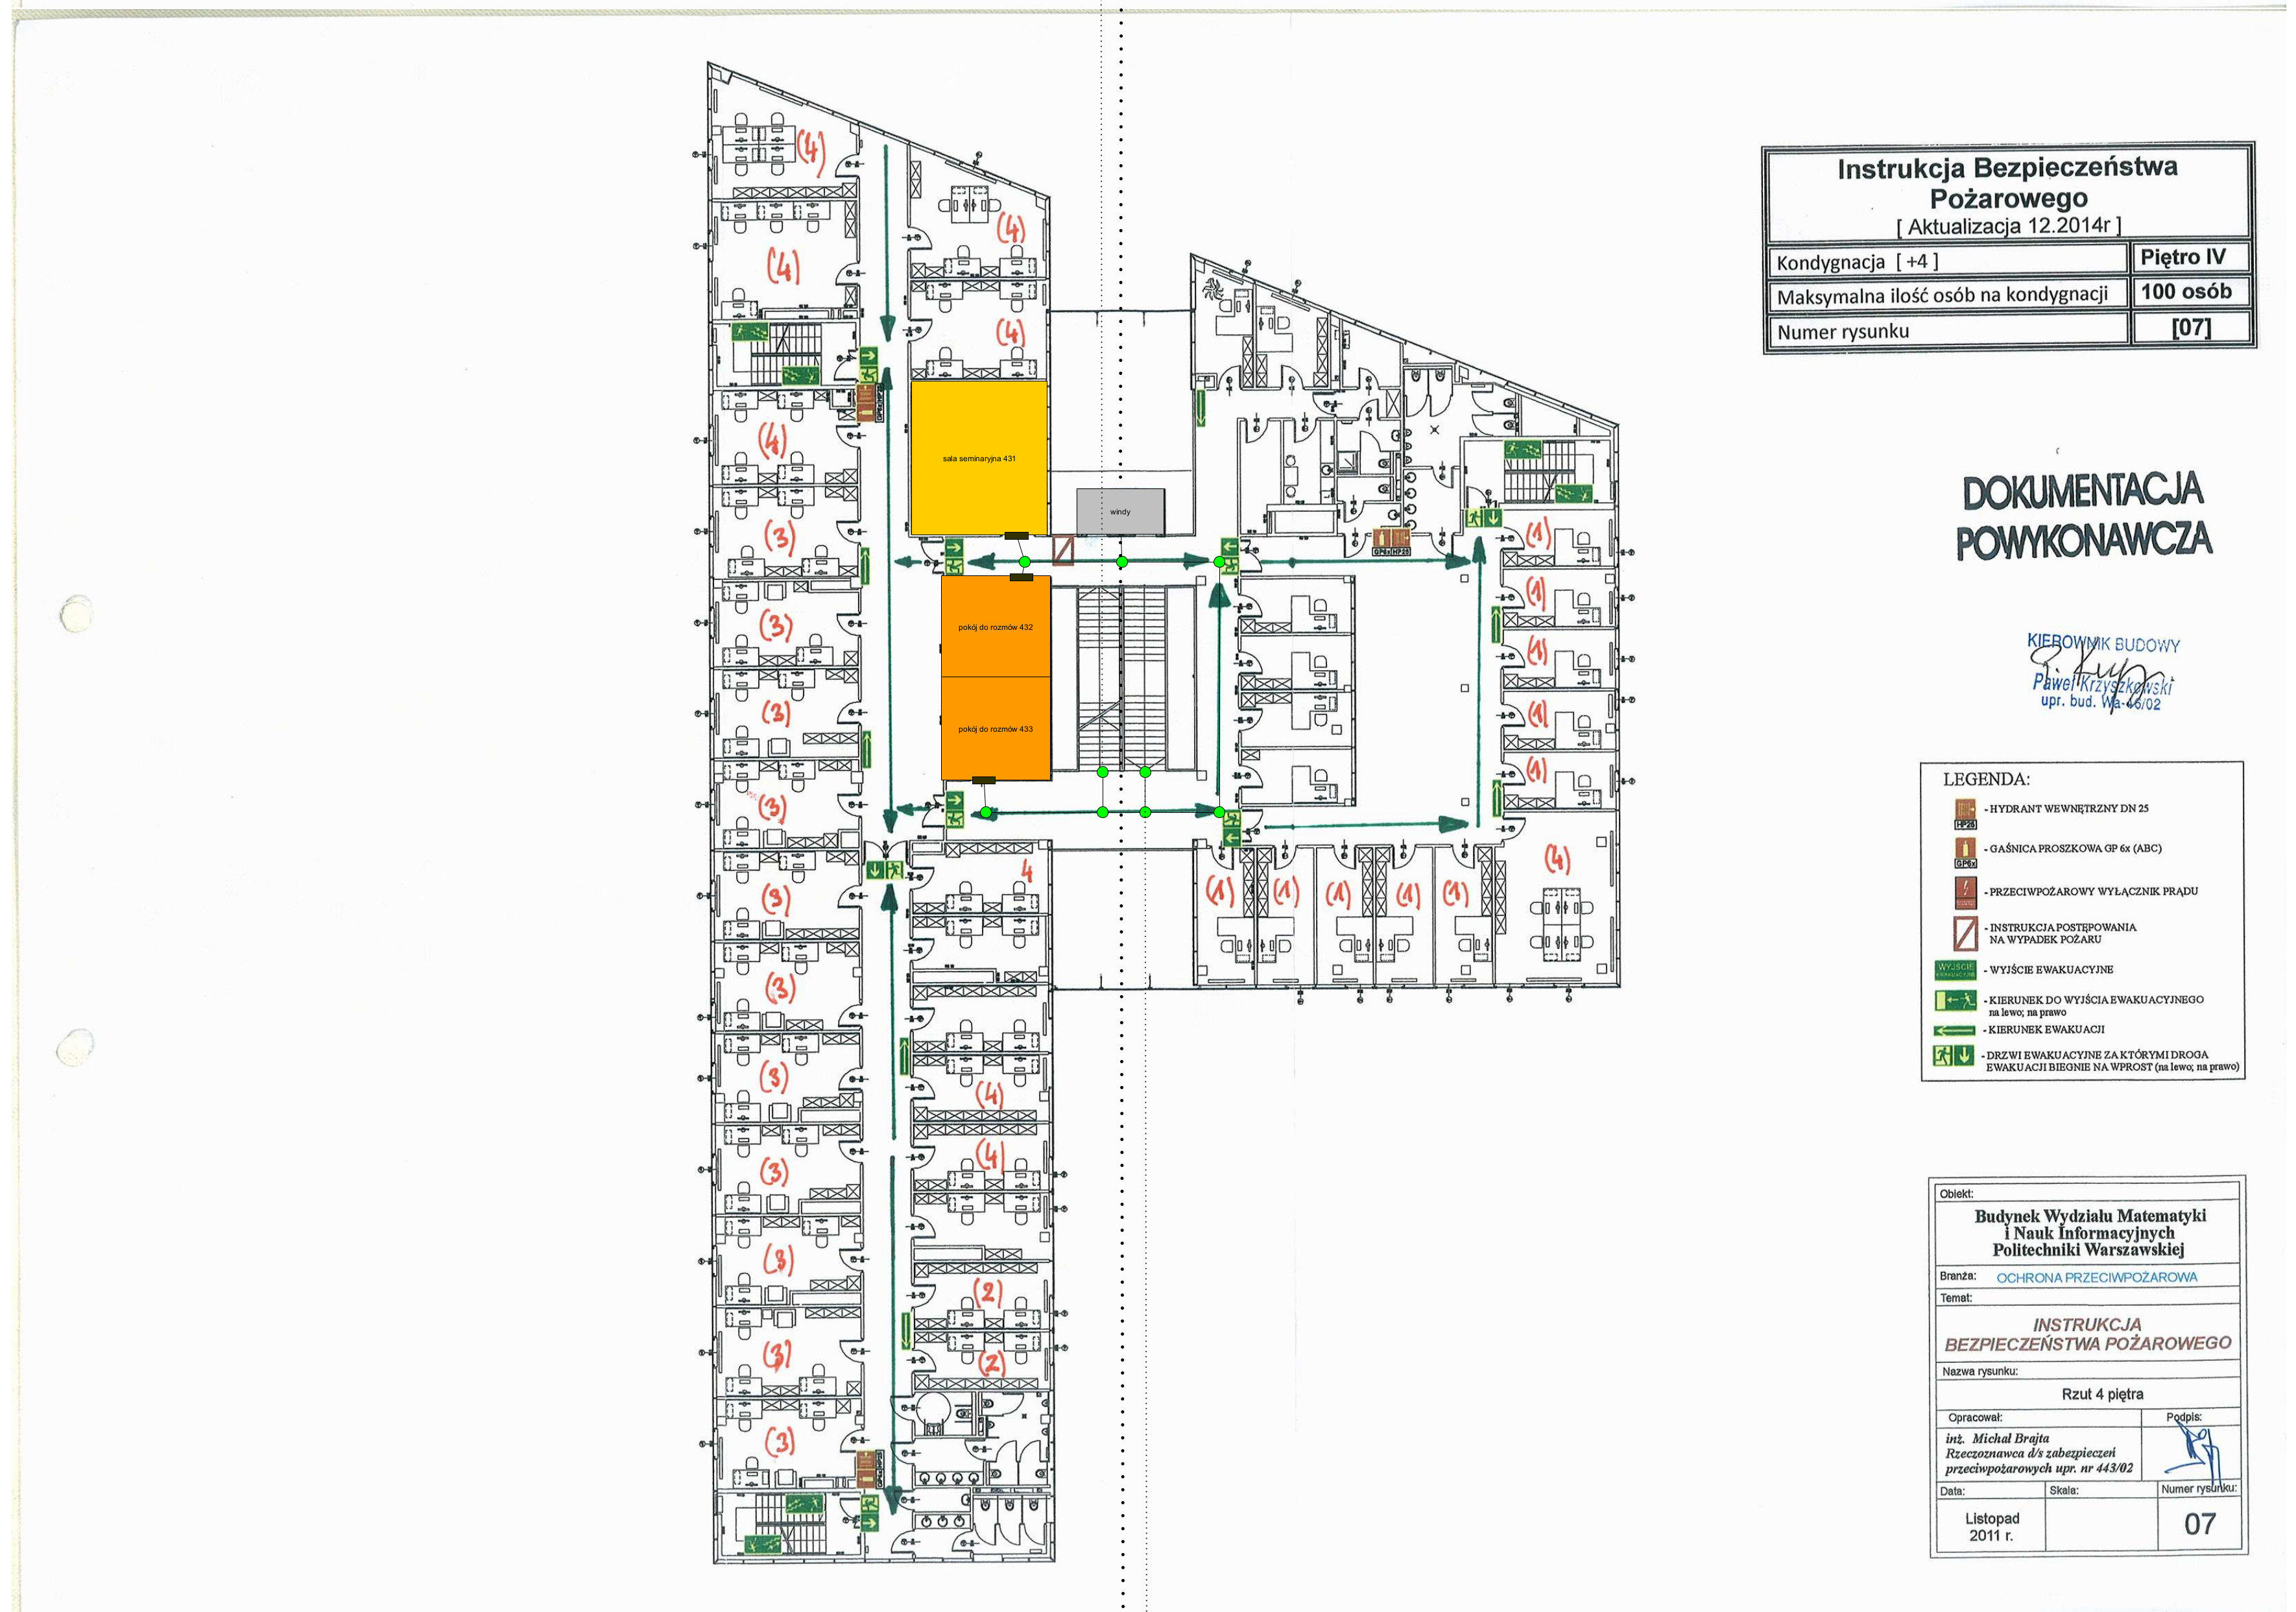
\includegraphics[width=\linewidth,height=0.22\textheight,keepaspectratio]{MINImapsGraf_2x1.png}
    \end{minipage}
    \caption{Piętro 4: plan ewakuacyjny przed wektoryzacją (po lewej) oraz plan po wektoryzacji (po prawej).}
    \label{fig:wektoryzacja-p4}
\end{figure}

\begin{figure}[t]
    \centering
    \begin{minipage}[t]{0.49\textwidth}
        \centering
        \includegraphics[width=\linewidth,height=0.22\textheight,keepaspectratio]{5pietro.png}
    \end{minipage}
    \hfill
    \begin{minipage}[t]{0.49\textwidth}
        \centering
        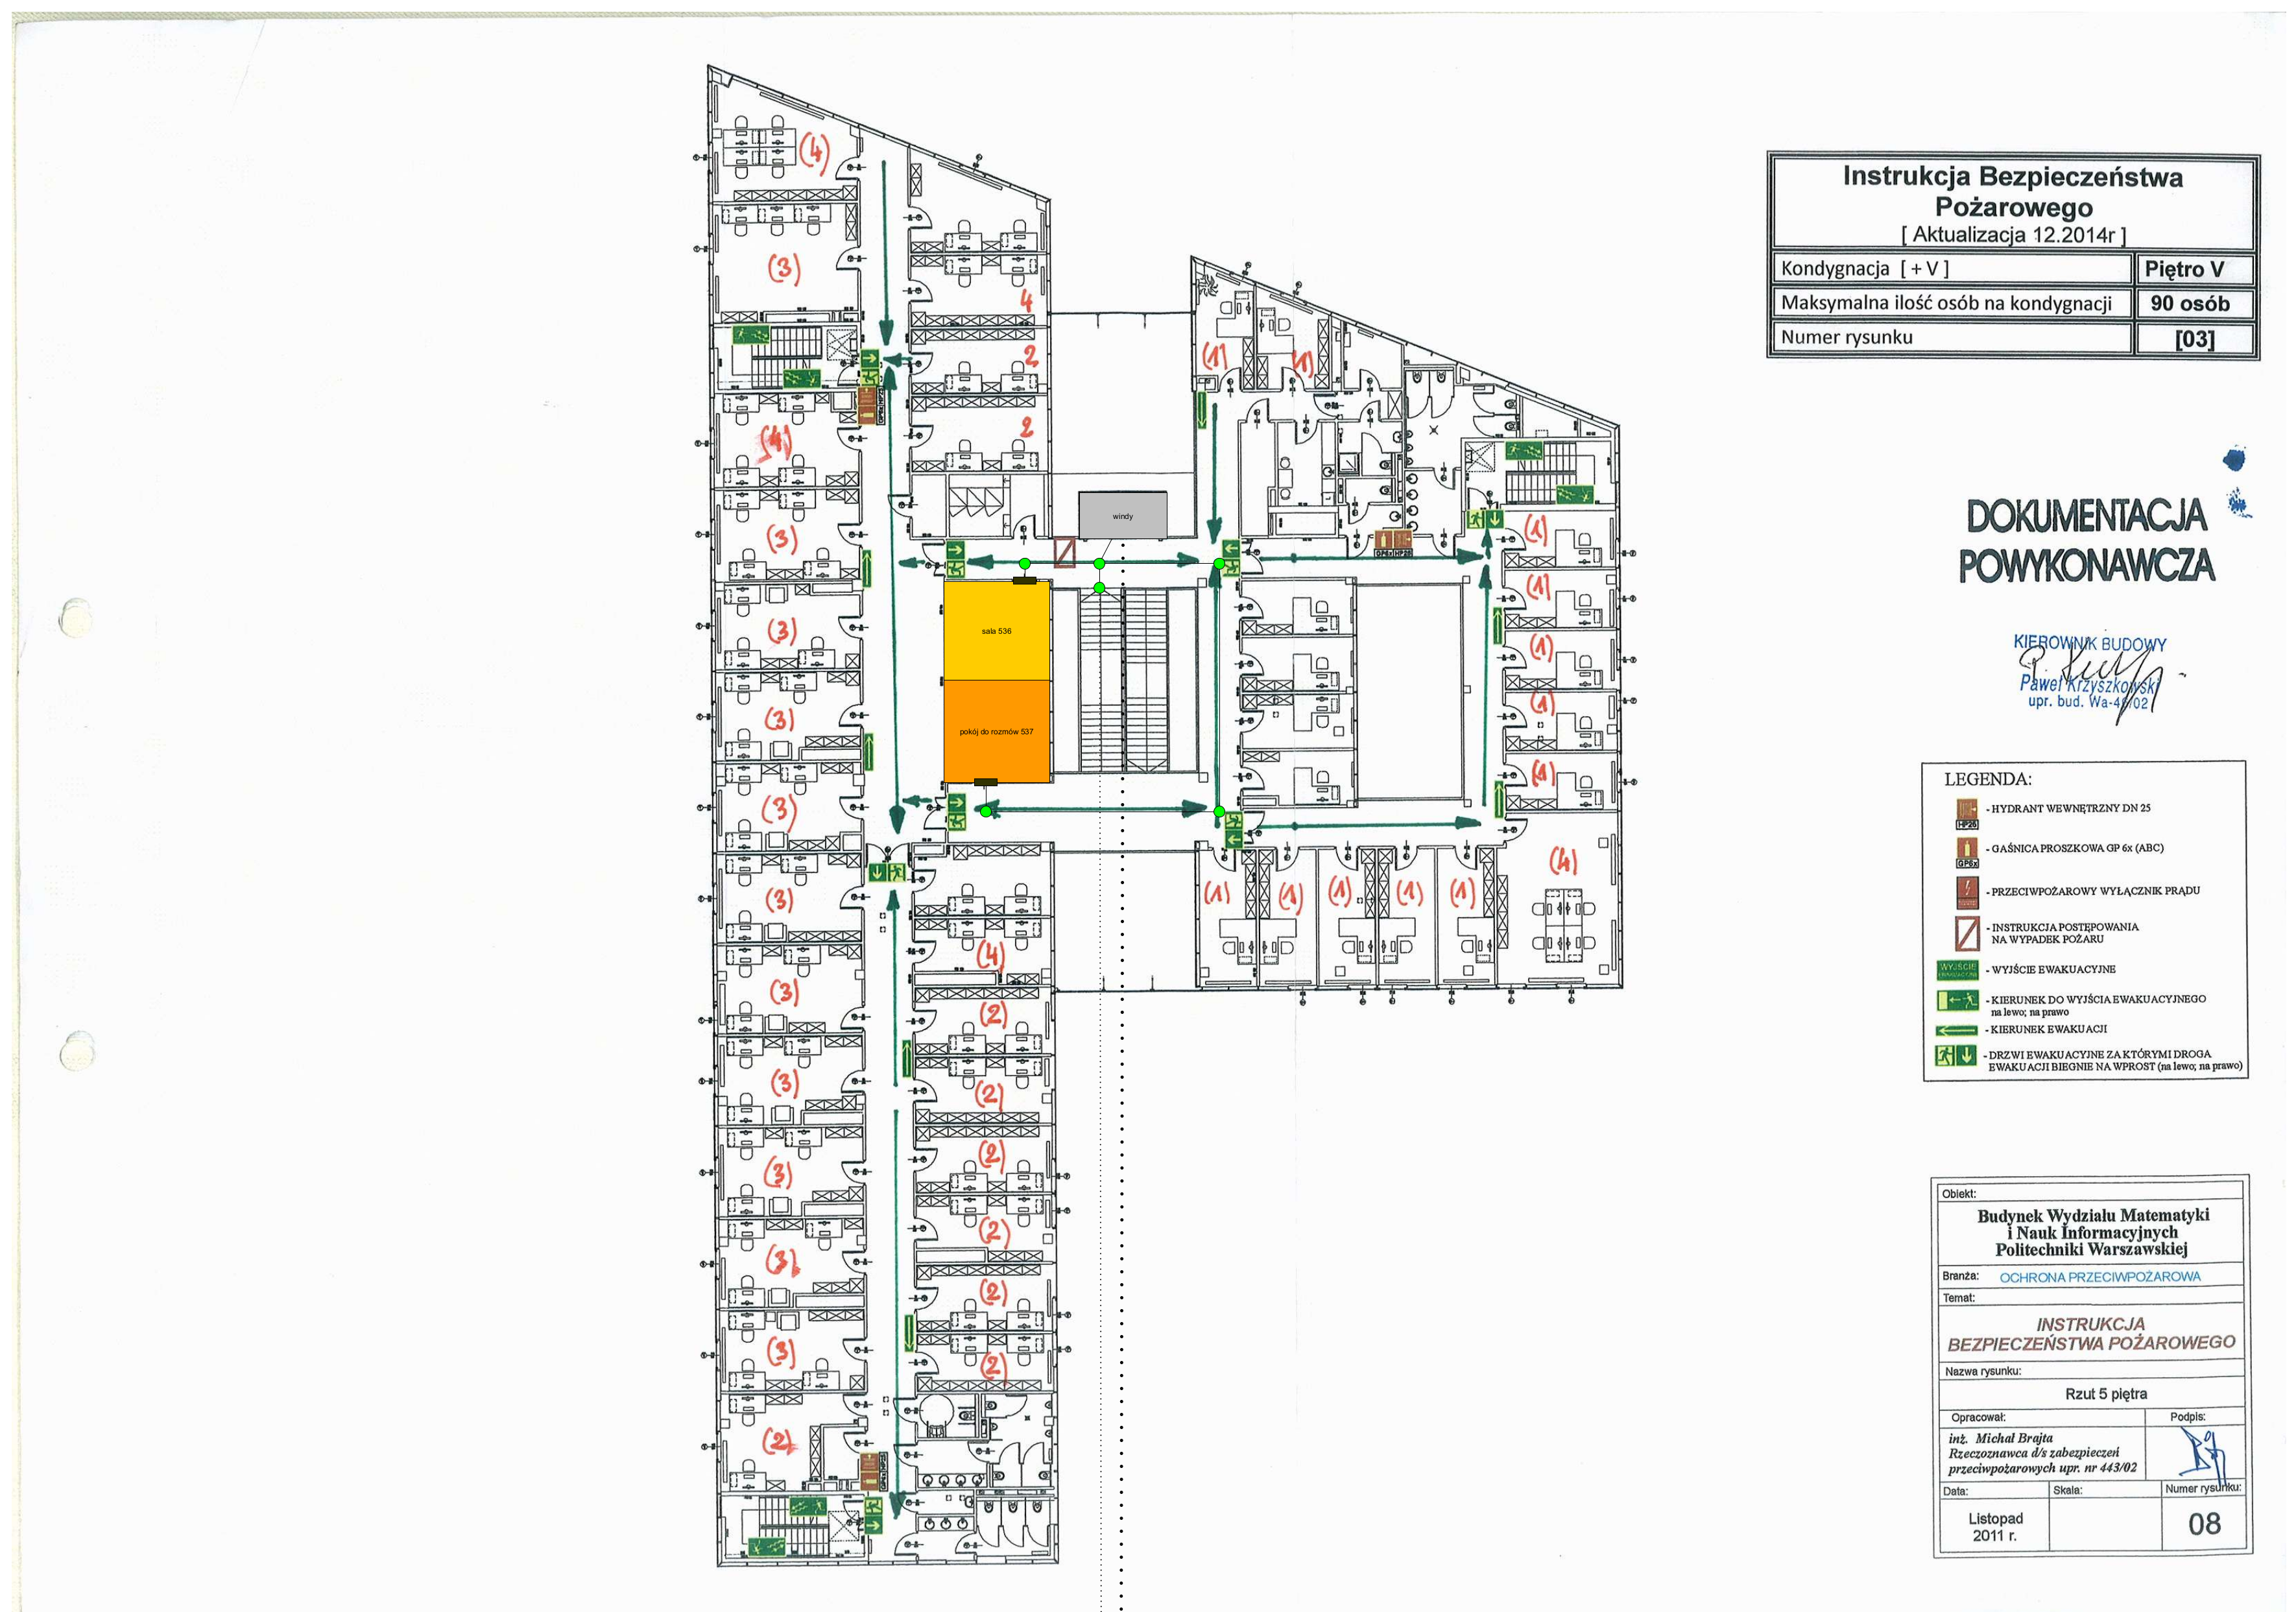
\includegraphics[width=\linewidth,height=0.22\textheight,keepaspectratio]{MINImapsGraf_1x1.png}
    \end{minipage}
    \caption{Piętro 5: plan ewakuacyjny przed wektoryzacją (po lewej) oraz plan po wektoryzacji (po prawej).}
    \label{fig:wektoryzacja-p5}
\end{figure}
\clearpage

\subsection{Wnioski}
Już podczas wstępnej analizy otrzymanych planów można zauważyć pierwsze problemy, jakie mogą wynikać z użytych przez nas metod. Nawet na niedużej skali jednego piętra liczba węzłów (zielonych kropek na rysunku) rośnie bardzo szybko, co znacząco zwiększa zasoby potrzebne przy obliczaniu optymalnych tras. W kontekście samego Wydziału MiNI nie jest to problem wymagający większej uwagi, jednak przy wykładniczym wzroście złożoności problemu wraz z dodawaniem kolejnych budynków może to mieć znaczący wpływ na odczucia z użytkowania aplikacji. W związku z tym w kolejnych etapach pracy nad projektem będzie to jeden z głównych tematów, na których będziemy się skupiać, jednak na ten moment nie jest to priorytet.

\subsection{POI (\textit{ang. points of interest - punkty zainteresowań})}
Ważną częścią naszych map będą tzw. POI, które każdy student powinien móc łatwo zlokalizować. Do takich miejsc zaliczane są przede wszystkim pokoje specjalne na wydziale, np. dziekanat, szatnia czy stołówka. Poza tym na mapie znajdą się specjalnie oznaczone miejsca z automatami do przekąsek, punktami druku dostępnymi dla studentów, a także miejscami wypoczynku i integracji studenckiej. Każdy taki punkt będzie posiadał krótki opis i link do informacji zamieszczonej na stronie wydziału \url{https://ww2.mini.pw.edu.pl}, a różne typy punktów zainteresowań będą oznaczone innym emblematem w celu łatwej identyfikacji. Punkty nanoszone na mapę będą początkowo przez nasz zespół, jednak z czasem użytkownicy będą mogli mieć możliwość dodawania własnych punktów, które będą musiały być akceptowane w celu uniknięcia szerzenia nieprawdziwych informacji.

\subsection{Informacje o parkingach}
Poza POI w samym budynku docelowo w aplikacji będą informacje o możliwości zaparkowania pojazdu wokół danego wydziału, wraz z ceną i przewidywaną dostępnością miejsc. Informacje te będą pobierane z ogólnodostępnych danych w Internecie, a także -- jeśli będzie taka możliwość -- z analizowania ruchu przy użyciu publicznych kamer. W przypadku Wydziału MiNI będzie osobna mapa piętra -1 wraz z danymi pozwalającymi na wynajęcie miejsca.

\subsection{Nawigowanie po zamkniętych przestrzeniach}
W ramach dalszego rozwoju projektu kluczowym wyzwaniem technologicznym będzie implementacja systemu pozycjonowania użytkownika wewnątrz gmachu MiNI, ponieważ klasyczny sygnał GPS nie zapewnia tam wystarczającej dokładności. Aby umożliwić nawigację w czasie rzeczywistym wzdłuż wyznaczonych już wektorów i węzłów grafu, rozważamy przetestowanie kilku systemów pozycjonowania wewnątrzbudynkowego (IPS). Podstawowym podejściem będzie próba wykorzystania istniejącej infrastruktury uczelnianej sieci Wi-Fi do przybliżonej lokalizacji. W celu uzyskania wyższej precyzji zbadamy również możliwości użycia nadajników Bluetooth Low Energy (BLE Beacons). Alternatywnie, najbardziej przystępnym rozwiązaniem na etapie wczesnych testów byłoby rozmieszczenie w strategicznych punktach wydziału kodów QR. Ich zeskanowanie przez użytkownika pozwoli na natychmiastowe skalibrowanie pozycji startowej w aplikacji, co stanowić będzie praktyczne dopełnienie zaprojektowanych algorytmów obliczających optymalne trasy i czas przejścia.

\section{Analiza przemieszczania się w obrębie jednego piętra}

\subsection{Cel i metodologia pomiarów}
W celu wyznaczenia jak najdokładniejszego ETA (\textit{ang. Estimated Time of Arrival - oczekiwany czas dotarcia do celu}) dla przeciętnego studenta, zebraliśmy grupę 10 osób reprezentujących społeczność Politechniki Warszawskiej. Wśród osób badanych było 5 kobiet oraz 5 mężczyzn z 1,2 i 3 roku studiów inżynierskich. Każda z badanych osób została poproszona o przejście 9 różnych dróg, osobno w jedną i w drugą stronę, swoim zwykłym tempem i zmierzenie czasu, jaki był im na to potrzebny. Trasy były wybierane w taki sposób, aby każda była innej długości i odzwierciedlała codzienne drogi, jakimi poruszają się studenci w trakcie dnia. Wszystkie trasy były w obrębie jednego piętra. Dane te zostały zebrane, a następnie dokonaliśmy obróbki w następujący sposób: odrzucono najniższy i najwyższy wynik jako możliwe odchylenia standardowe, a następnie policzono średni wynik. Jako względny błąd pomiarowy przyjęto $\pm 10\%$; wynika to z wielu możliwych czynników, jakie wpływają na ostateczny wynik. Podczas późniejszego wywiadu z badanymi za główny powód odchyleń wskazano znaczącą ilość osób przebywających na terenie.

\subsection{Wyniki pomiarów}
Poniżej przedstawiono wyniki przeprowadzonego badania w tabeli wraz z błędem bezwzględnym dla każdej trasy oraz jej średnią długością. Wartości odległości wyznaczyłyśmy samodzielnie, korzystając z dostępnych metod pomiarowych w terenie. W każdym wierszu na czerwono zaznaczono wartość minimalną i maksymalną, a średni czas obliczono po odrzuceniu tych dwóch skrajnych wyników.

\begin{table}[H]
\centering
\caption{Wyniki badań w obrębie jednego piętra -- Tabela 1}
\label{tab:wyniki-jedno-pietro}
\scriptsize
\setlength{\tabcolsep}{1.5pt}
\renewcommand{\arraystretch}{1.2}
\setlength{\arrayrulewidth}{0.5pt}
\setlength{\doublerulesep}{0pt}
\begin{tabular}{|>{\centering\arraybackslash}m{3.1cm}|c|cccccccccc|c|c|}
\hline
\textbf{Trasa} & \textbf{\shortstack{Odległość\\{[m]}}} & \textbf{P1 [s]} & \textbf{P2 [s]} & \textbf{P3 [s]} & \textbf{P4 [s]} & \textbf{P5 [s]} & \textbf{P6 [s]} & \textbf{P7 [s]} & \textbf{P8 [s]} & \textbf{P9 [s]} & \textbf{P10 [s]} & \textbf{\shortstack{Średni\\czas [s]}} & \textbf{\shortstack{Błąd\\bezwzgl. [s]}} \\
\hline
Szatnia --\\Prodziekanat & 22 & 17,19 & 17,92 & 18,36 & 16,10 & \textcolor{red}{18,90} & 16,14 & 17,78 & \textcolor{red}{15,79} & 18,08 & 15,99 & 17,20 & $\pm$1,72 \\
\hline
Dziekanat --\\Stołówka & 42 & 32,29 & 33,62 & 33,74 & 34,01 & 31,91 & 34,65 & \textcolor{red}{35,44} & \textcolor{red}{29,81} & 32,40 & 35,25 & 33,48 & $\pm$3,35 \\
\hline
Łazienka -- 107 & 8 & 6,27 & 6,57 & 6,20 & 6,02 & \textcolor{red}{6,84} & \textcolor{red}{5,75} & 6,60 & 6,70 & 5,84 & 6,05 & 6,28 & $\pm$0,63 \\
\hline
213 -- Łazienka p.2\\przy windzie & 26 & 20,58 & 19,78 & 20,75 & 20,03 & 22,20 & \textcolor{red}{22,33} & 19,82 & 22,20 & \textcolor{red}{18,81} & 18,92 & 20,54 & $\pm$2,05 \\
\hline
212 -- Łazienka p.2\\przy laboratoriach & 31 & 24,43 & 25,24 & 25,89 & 25,99 & \textcolor{red}{26,83} & 26,19 & 23,29 & 25,62 & 26,50 & \textcolor{red}{22,44} & 25,39 & $\pm$2,54 \\
\hline
Automat z napojami (lewo) --\\Winda p.3 & 21 & 16,33 & 16,31 & 15,20 & 15,16 & 16,26 & 16,89 & 17,88 & \textcolor{red}{15,13} & 16,35 & \textcolor{red}{17,95} & 16,30 & $\pm$1,63 \\
\hline
Winda p.4 --\\Pokój rozmów & 4 & 3,79 & 3,99 & 3,81 & \textcolor{red}{3,59} & 3,89 & 3,61 & 3,90 & 3,90 & 3,71 & \textcolor{red}{4,01} & 3,83 & $\pm$0,38 \\
\hline
316 -- 313 & 14 & 11,03 & 10,82 & 10,96 & 11,76 & 10,48 & \textcolor{red}{10,34} & 11,19 & 10,89 & \textcolor{red}{11,86} & 10,48 & 10,95 & $\pm$1,09 \\
\hline
Bilard --\\Drzwi WRS MiNI & 38 & 29,57 & 28,81 & 26,95 & 29,28 & 28,46 & 29,27 & 31,13 & \textcolor{red}{26,83} & \textcolor{red}{32,46} & 30,82 & 29,29 & $\pm$2,93 \\
\hline
\end{tabular}
\renewcommand{\arraystretch}{1.0}
\end{table}

\begin{figure}[H]
    \centering
    \begin{tikzpicture}
        \begin{axis}[
            width=13.2cm,
            height=8.4cm,
            xlabel={Odległość trasy [m]},
            ylabel={Czas przejścia [s]},
            xmin=0, xmax=45,
            ymin=0, ymax=40,
            grid=major,
            major grid style={dashed, gray!30},
            minor tick num=1,
            legend style={at={(0.03,0.97)}, anchor=north west, font=\footnotesize, fill=white, draw=gray!40},
            title={Pomiary czasu przejścia względem odległości (bez wartości skrajnych)}
        ]
            % Punkty pomiarowe po odrzuceniu wartości minimalnej i maksymalnej (zaznaczonych na czerwono w tabeli).
            \addplot[
                only marks,
                mark=*,
                mark size=1.6pt,
                color=blue!70!black
            ] coordinates {
                (22,17.19) (22,17.92) (22,18.36) (22,16.10) (22,16.14) (22,17.78) (22,18.08) (22,15.99)
                (42,32.29) (42,33.62) (42,33.74) (42,34.01) (42,31.91) (42,34.65) (42,32.40) (42,35.25)
                (8,6.27) (8,6.57) (8,6.20) (8,6.02) (8,6.60) (8,6.70) (8,5.84) (8,6.05)
                (26,20.58) (26,19.78) (26,20.75) (26,20.03) (26,22.20) (26,19.82) (26,22.20) (26,18.92)
                (31,24.43) (31,25.24) (31,25.89) (31,25.99) (31,26.19) (31,23.29) (31,25.62) (31,26.50)
                (21,16.33) (21,16.31) (21,15.20) (21,15.16) (21,16.26) (21,16.89) (21,17.88) (21,16.35)
                (4,3.79) (4,3.99) (4,3.81) (4,3.89) (4,3.61) (4,3.90) (4,3.90) (4,3.71)
                (14,11.03) (14,10.82) (14,10.96) (14,11.76) (14,10.48) (14,11.19) (14,10.89) (14,10.48)
                (38,29.57) (38,28.81) (38,26.95) (38,29.28) (38,28.46) (38,29.27) (38,31.13) (38,30.82)
            };
            \addlegendentry{Punkty pomiarowe (bez min/max)}

            \addplot[
                blue!80!black,
                thick,
                domain=0:45
            ] {0.7837093*x + 0.2017649};
            \addlegendentry{Linia trendu (regresja liniowa)}

            \addplot[
                red!80!black,
                dashed,
                thick,
                domain=0:45
            ] {0.70524795*x + 0.1843246};
            \addlegendentry{Trend minimalny}

            \addplot[
                red!80!black,
                dashed,
                thick,
                domain=0:45
            ] {0.86217065*x + 0.21920521};
            \addlegendentry{Trend maksymalny}
        \end{axis}
    \end{tikzpicture}
    \caption{Zależność czasu przejścia od odległości na jednym piętrze. Na wykresie uwzględniono wszystkie punkty poza skrajnymi (oznaczonymi na czerwono w Tabeli 1) oraz linie trendu: średnią, minimalną i maksymalną.}
    \label{fig:regresja-jedno-pietro}
\end{figure}

\subsection{Analiza wyników}
Celem pierwszej próby badawczej było ustalenie średniej prędkości, z jaką student porusza się w obrębie jednego piętra. Przy użyciu narzędzi regresji liniowej dla wielu wyników ustaliliśmy, że średnia prędkość studenta na wydziale wynosi ok.:
\begin{equation}
    v_{\text{sr}} \approx 1{,}3\ \text{m/s} \quad (\approx 4{,}7\ \text{km/h})
\end{equation}
Wartość ta została przyjęta w modelu jako domyślna prędkość ruchu użytkownika na odcinkach poziomych.

Dodatkowo analiza wykresu z Rysunku \ref{fig:regresja-jedno-pietro} pokazuje, że zależność czasu od odległości jest bardzo bliska liniowej w całym badanym zakresie. Punkty pomiarowe (po odrzuceniu skrajnych wartości oznaczonych wcześniej na czerwono) układają się wzdłuż prostej trendu bez widocznych odchyleń systematycznych dla krótkich i długich tras, co potwierdza, że przy ruchu po jednym piętrze najistotniejszym czynnikiem jest dystans.

W modelu uwzględniono trzy linie trendu: linię średnią, linię minimalną oraz linię maksymalną. Linia średnia reprezentuje typowy czas przejścia, natomiast linie minimalna i maksymalna wyznaczają praktyczny przedział zmienności wyników obserwowanych w pomiarach terenowych. Takie podejście pozwala nie tylko oszacować pojedynczą wartość ETA, ale też zbudować wiarygodny zakres czasowy przejścia dla użytkowników o różnym tempie ruchu i przy różnym chwilowym natężeniu ruchu na korytarzu.

\subsection{Wnioski i zastosowanie}
Wyniki otrzymane podczas próby badawczej stanowią podstawę budowy algorytmu liczącego czas trasy z punktu A do punktu B. Wyznaczony podczas badania czas będzie rozkładany na wektory łączące dane węzły. Wstępne założenia i wyniki wskazują, że średni czas przejścia pomiędzy dwoma węzłami na tym samym piętrze jest liniowo zależny od sumy odległości.

W kontekście MINI Maps oznacza to, że dla każdej krawędzi grafu można przypisać wagę czasową wyznaczaną na podstawie regresji liniowej, a następnie sumować ją wzdłuż całej trasy. W trybie podstawowym aplikacja może korzystać z linii średniej (najbardziej prawdopodobny czas), a w trybie rozszerzonym prezentować także zakres ,,optymistyczny--pesymistyczny'' wynikający z linii minimalnej i maksymalnej. Dzięki temu użytkownik otrzymuje nie tylko jedno ETA, ale też realną informację o możliwym rozrzucie czasu dojścia.

Tak przygotowany model poprawia jakość nawigacji szczególnie podczas krótkich przerw między zajęciami, kiedy nawet niewielkie odchylenia czasu mają znaczenie praktyczne. Jednocześnie sytuację nadal komplikują schody i winda, gdzie wybór pomiędzy jednym a drugim środkiem przemieszczania istotnie wpływa na całkowity czas przejścia i wymaga osobnego modelowania dla ruchu między piętrami.

\section{Analiza czasu przemieszczania między piętrami}

\subsection{Cel i metodologia pomiarów}
W wielopiętrowym gmachu Wydziału MiNI jednym z największych wyzwań dla studentów jest szybkie przemieszczanie się między kondygnacjami, szczególnie podczas krótkich 15-minutowych przerw. Aby nasza aplikacja mogła rzetelnie wyznaczać najszybsze trasy, nie mogliśmy polegać na samych domysłach czy planach architektonicznych. Konieczne było zebranie rzeczywistych danych. W tym celu przeprowadziliśmy pomiary terenowe, badając realny czas podróży windą oraz klatkami schodowymi.

\subsection{Pomiary windy: przejazd z poziomu 0 na 5 piętro}
Na początku skupiliśmy się wyłącznie na windzie i wykonaliśmy serię niezależnych pomiarów pełnego przejazdu na dystansie od poziomu 0 do 5 piętra (bez doliczania czasu oczekiwania na przyjazd kabiny). Uzyskane czasy przedstawiono poniżej:
\begin{itemize}
    \item Pomiar 1: 39 s
    \item Pomiar 2: 41 s
    \item Pomiar 3: 40 s
    \item Pomiar 4: 42 s
    \item Pomiar 5: 38 s
    \item Pomiar 6: 40 s
\end{itemize}

Średni czas przejazdu z sześciu prób wyniósł dokładnie \textbf{40 sekund}. Rozrzut wyników (38--42 s) jest niewielki, więc do dalszego modelowania przyjęliśmy wartość 40 s jako reprezentatywną dla przejazdu 0 $\rightarrow$ 5.

\begin{figure}[H]
    \centering
    \begin{tikzpicture}
        \begin{axis}[
            width=12cm, height=7cm,
            ybar,
            bar width=12pt,
            xlabel={Numer pomiaru},
            ylabel={Czas przejazdu [sekundy]},
            xmin=0.5, xmax=6.5,
            ymin=35, ymax=44,
            xtick={1,2,3,4,5,6},
            grid=major,
            major grid style={dashed, gray!30},
            title={Czas przejazdu windy na trasie 0 $\rightarrow$ 5}
        ]
        \addplot[fill=blue!45] coordinates {
            (1,39) (2,41) (3,40) (4,42) (5,38) (6,40)
        };
        \addplot[red, thick, domain=0.5:6.5] {40};
        \end{axis}
    \end{tikzpicture}
    \caption{Wyniki serii pomiarów czasu przejazdu windy z poziomu 0 na 5 piętro. Czerwona linia oznacza średnią równą 40 s.}
    \label{fig:pomiary-windy-0-5}
\end{figure}

\subsection{Wnioski z pomiarów windy}
Seria pomiarów pokazała, że całkowity czas przejazdu windy na dystansie 0 $\rightarrow$ 5 (łącznie z wejściem i wyjściem) jest stabilny i wynosi około 40 s. Ponieważ z obserwacji terenowych wynika, że sam narzut wejścia/wyjścia to ok. 20 s, czas ruchu kabiny wynosi ok. 20 s na 5 pięter, czyli \textbf{4 sekundy na jedno piętro}.

\subsection{Dokumentacja fotograficzna punktów pomiarowych}
Aby uwiarygodnić zebrane dane i pokazać kontekst przestrzenny pomiarów, do raportu dołączono dokumentację fotograficzną dwóch kluczowych punktów komunikacji pionowej na Wydziale MiNI: głównej klatki schodowej oraz windy. Zdjęcia przedstawiają rzeczywiste miejsca, w których wykonywano pomiary czasów przejścia i przejazdu.

\begin{figure}[H]
    \centering
    \begin{minipage}[t]{0.48\textwidth}
        \centering
        \includegraphics[width=\textwidth]{/Users/marcinpawlak/.cursor/projects/Users-marcinpawlak-Documents-STUDIA-SEM-2-minimaps/assets/IMG_4345-1c295508-a341-4225-95ec-721e864afc77.png}
        {\small (a) Główna klatka schodowa -- punkt odniesienia dla pomiarów ruchu pieszego.\par}
    \end{minipage}
    \hfill
    \begin{minipage}[t]{0.48\textwidth}
        \centering
        \includegraphics[width=\textwidth]{/Users/marcinpawlak/.cursor/projects/Users-marcinpawlak-Documents-STUDIA-SEM-2-minimaps/assets/IMG_4344-d5bd4d73-9aaf-4d81-bc1d-c2ea0667129e.png}
        {\small (b) Winda osobowa -- punkt pomiaru czasu przejazdu i narzutu wejścia/wyjścia.\par}
    \end{minipage}
\end{figure}

\subsection{Zebranie danych surowych}
Do modelu porównawczego zebraliśmy następujące dane:
\begin{itemize}
    \item \textbf{Całkowity czas przejazdu windą (z poziomu 0 na 5 piętro):} 40 sekund.
    \item \textbf{Średni czas narzutu dla windy (wsiadanie i wysiadanie):} 20 sekund.
    \item \textbf{Czas wejścia po schodach (1 piętro):} około 12 sekund (zakładając typowe studenckie tempo).
\end{itemize}

\subsection{Przetwarzanie danych: uproszczony model czasowy}
Aby nasza aplikacja mogła dynamicznie porównywać oba warianty tras, musieliśmy przekształcić zebrane dane w prosty model.

W pierwszej kolejności rozdzieliliśmy czas całkowity windy na część stałą i część zależną od liczby pięter. Skoro pełny przejazd 0 $\rightarrow$ 5 trwa 40 s, a 20 s stanowi narzut wejścia/wyjścia, to na sam ruch kabiny pozostaje 20 s. Oznacza to \textbf{4 sekundy na jedno piętro}.

Na tej podstawie możemy zestawić przewidywany czas podróży obu metod w zależności od liczby pięter:
\begin{itemize}
    \item \textbf{Całkowity czas dla windy} to 20 sekund stałego narzutu wejścia/wyjścia plus 4 sekundy za każde pokonywane piętro.
    \item \textbf{Całkowity czas dla schodów} to po prostu 12 sekund pomnożone przez liczbę pięter.
\end{itemize}

\subsection{Analiza wyników: gdzie jest punkt opłacalności?}
Po przyjęciu modelu opartego na rzeczywistym czasie przejazdu (40 s na dystansie 0 $\rightarrow$ 5, łącznie z wejściem i wyjściem), porównaliśmy oba warianty dla faktycznego zakresu budynku, czyli od 1 do 5 pięter:

\begin{itemize}
    \item \textbf{Pokonanie 1 piętra:} Winda to ok. 24 sekundy, schody to 12 sekund. (Szybsze są schody).
    \item \textbf{Pokonanie 2 pięter:} Winda to ok. 28 sekund, schody to 24 sekundy. (Nadal szybsze są schody).
    \item \textbf{Pokonanie 3 pięter:} Winda to ok. 32 sekundy, schody to 36 sekund. (Szybsza jest winda).
    \item \textbf{Pokonanie 5 pięter:} Winda to ok. 40 sekund, schody to 60 sekund. (Wyraźnie szybsza jest winda).
\end{itemize}

\subsection{Wnioski dla algorytmu nawigacji}
Powyższe zestawienie dostarcza nam gotowego rozwiązania, które zostanie bezpośrednio zaimplementowane w kodzie aplikacji MiniMaps.

Otrzymaliśmy wynik: dla 1--2 pięter \textbf{szybsze są schody}, a od 3 pięter \textbf{szybsza jest winda}.

Dzięki takiemu rozwiązaniu system ograniczy liczbę nietrafionych podpowiedzi i będzie lepiej odzwierciedlał realne warunki poruszania się po wydziale. Oczywiście w ustawieniach aplikacji może pozostać opcja preferowania schodów (np. z powodów zdrowotnych, sportowych lub przy dużym obciążeniu windy).

\subsection{Weryfikacja matematyczna i wizualizacja modelu}

Aby poprzeć powyższe obserwacje twardymi dowodami, przekształciliśmy zebrane czasy w prosty model matematyczny. Pozwala on aplikacji na płynne przeliczanie opłacalności trasy.

Czas przemieszczania się klatką schodową ($T_s$) w funkcji pokonywanych pięter ($n$) jest funkcją liniową rosnącą w tempie 12 sekund na kondygnację:
\begin{equation}
    T_s(n) = 12n
\end{equation}

Z kolei całkowity czas podróży windą ($T_w$) to suma stałego narzutu 20 s (wejście i wyjście) oraz czasu przejazdu 4 s na każde pokonywane piętro:
\begin{equation}
    T_w(n) = 20 + 4n
\end{equation}

Sprawdzamy teraz punkt przecięcia obu funkcji:
\begin{equation}
    12n = 20 + 4n \implies 8n = 20 \implies n = 2{,}5
\end{equation}

Przecięcie występuje przy $n=2{,}5$, co oznacza, że dla 1--2 pięter korzystniejsze czasowo są schody, a od 3 pięter korzystniejsza staje się winda. Pełne zestawienie dla zakresu 1--5 pięter ilustruje poniższy wykres (Rysunek \ref{fig:wykres-windy}).

\begin{figure}[H]
    \centering
    \begin{tikzpicture}
        \begin{axis}[
            width=12cm, height=8cm,
            xlabel={Liczba pięter do pokonania ($n$)},
            ylabel={Szacowany czas [sekundy]},
            xmin=1, xmax=5,
            ymin=0, ymax=65,
            xtick={1,2,3,4,5},
            legend pos=north west,
            grid=major,
            major grid style={dashed, gray!30},
            title={Winda czy schody? Analiza opłacalności czasu transportu}
        ]
        \addplot[
            color=blue,
            mark=square*,
            line width=1.5pt
        ] coordinates {
            (1, 24) (2, 28) (3, 32) (4, 36) (5, 40)
        };
        \addlegendentry{Winda (20 s narzutu + 4 s/piętro)}

        \addplot[
            color=red,
            mark=*,
            line width=1.5pt
        ] coordinates {
            (1, 12) (2, 24) (3, 36) (4, 48) (5, 60)
        };
        \addlegendentry{Schody}

        \node[label={270:{Punkt opłacalności (2,5 piętra)}},circle,fill,inner sep=2pt, color=black] at (axis cs:2.5,30) {};
        \end{axis}
    \end{tikzpicture}
    \caption{Zależność szacowanego czasu dotarcia na zajęcia od wybranego środka transportu pionowego w zakresie 1--5 pięter. Wykres pokazuje, że przy uwzględnieniu 20 s narzutu wejścia/wyjścia schody są szybsze dla 1--2 pięter, natomiast od 3 pięter szybsza staje się winda.}
    \label{fig:wykres-windy}
\end{figure}

\section{Podsumowanie i dalszy rozwój}

Pierwsze wyniki badań są obiecujące i pokazują, że istnieje realne zapotrzebowanie na aplikację pomagającą studentom odnaleźć się na kampusie PW. Zebrane w trakcie pomiarów dane będą podstawą działania algorytmów znajdowania tras i wyznaczania czasu potrzebnego studentom na przemieszczenie się pomiędzy salami, a wyniki ankiet jasno wskazują kierunek, w jakim aplikacja powinna się rozwijać. Niestety jednak wstępna wektoryzacja planów ewakuacyjnych i problem lokalizacji użytkownika na zamkniętym obszarze ukazują już na tak wczesnym etapie problemy konstrukcyjne, nad których rozwiązaniem będą skupiać się kolejne raporty. Plan na dalszy rozwój obejmuje m.in. opracowanie działającego prototypu map na MiNI, rozwinięcie działania na inne wydziały oraz połączenie z już istniejącymi aplikacjami, tzn. Google Maps oraz Apple Maps, aby móc nawigować do budynków PW poza Kampusem, np. domów studenckich bądź miejsc spotkań na zajęcia z WF-u.

\section{Podział prac w zespole}

\begin{itemize}
    \item Goran Pangełow -- redakcja raportu.
    \item Marcin Pawlak -- analiza czasu przejazdu windą i schodami.
    \item Mikołaj Pesta -- wektoryzacja map.
    \item Ignacy Drężek -- analiza danych.
    \item Iga Oleksiewicz -- przygotowanie i realizacja ankiet.
    \item Maks Młynarczyk -- badanie przemieszczania się w obrębie jednego piętra.
\end{itemize}

\end{document}
